%  MDPI Electronics submission
%  Converted from the TMIS manuscript TMIS-09-2026-0123.
%  Compile with: pdflatex manuscript && pdflatex manuscript
%=================================================================
\documentclass[electronics,article,submit,pdftex,oneauthor]{Definitions/mdpi}

%=================================================================
\firstpage{1}
\makeatletter
\setcounter{page}{\@firstpage}
\makeatother
\pubvolume{1}
\issuenum{1}
\articlenumber{0}
\pubyear{2026}
\copyrightyear{2026}
\datereceived{ }
\daterevised{ }
\dateaccepted{ }
\datepublished{ }
\hreflink{https://doi.org/}

%=================================================================
% Additional packages and macros
\usepackage{amssymb}
\newcommand{\D}{\varDelta}                 % italic capital Delta (parameter displacement)
\newcommand{\E}{\mathbb{E}}
\newcommand{\phibar}{\bar{\phi}}
\newcommand{\Neff}{N_{\mathrm{eff}}}
\newcommand{\cRAG}{c_{\mathrm{RAG}}}
\newcommand{\Gmax}{G_{\max}}
\newcommand{\tkm}{t_k^{-}}
\newcommand{\tkp}{t_k^{+}}
\newcommand{\calA}{\mathcal{A}}
\newcommand{\calC}{\mathcal{C}}
\newcommand{\calX}{\mathcal{X}}
\newcommand{\calD}{\mathcal{D}}
\newcommand{\calW}{\mathcal{W}}

%=================================================================
% Full title of the paper (Capitalized)
\Title{Mathematical Modeling of Large Language Model Maintenance: A Stochastic Optimal-Control Framework for Retraining Scheduling, Knowledge Retention, and Alignment Preservation}

% MDPI internal command: Title for citation in the left column
\TitleCitation{Mathematical Modeling of Large Language Model Maintenance}

% Author Orchid ID: enter ID or remove command
%\newcommand{\orcidauthorA}{0000-0000-0000-000X} % Add \orcidA{} behind the author's name

% Authors, for the paper (add full first names)
\Author{Ook Lee}

% MDPI internal command: Authors, for metadata in PDF
\AuthorNames{Ook Lee}

% MDPI internal command: Authors, for citation in the left column
\AuthorCitation{Lee, O.}

% Affiliations / Addresses (Add [1] after \address if there is only one affiliation.)
\address[1]{Department of Information Systems, Hanyang University, Seoul 04763, Republic of Korea; ooklee@hanyang.ac.kr}

% Contact information of the corresponding author
\corres{Correspondence: ooklee@hanyang.ac.kr}

% Abstract (MDPI: single paragraph of about 200 words maximum)
\abstract{Large language models (LLMs) are deployed as long-lived software artifacts whose usefulness degrades as the world drifts away from their training distribution, yet they are still largely maintained by fixed calendars and ad hoc judgment. This paper treats a deployed LLM as a deteriorating system and casts its maintenance---when, how, and how much to update it---as a constrained stochastic optimal-control problem. Loss of freshness is modeled as a shock-and-wear process driven by drift events, update-induced catastrophic forgetting as a Fisher-information-weighted quadratic penalty interpreted as imperfect maintenance, and update cost as scaling with model and data size. Scheduling is formulated as an average-cost Markov decision process whose optimal policy, under stochastic-monotonicity and submodularity conditions, escalates monotonically through a graduated menu of maintenance actions. Retrieval-augmented generation is characterized as a feedback compensator, with a closed-form condition under which blending it with parametric maintenance dominates either alone. A square-root law links update cost, drift intensity, and the optimal maintenance interval, and lower forgetting per event is shown to warrant more frequent maintenance. A case study on a public pretrained model confirms affine staleness growth, recovers a retrieval-absorbed drift share equal to retrieval coverage, and shows that unreplayed low-rank adaptation can be dominated by taking no action.}

% Keywords (3 to 10)
\keyword{large language models; model maintenance; catastrophic forgetting; concept drift; condition-based maintenance; continual learning; Markov decision processes; renewal theory}

%=================================================================
\begin{document}

%-----------------------------------------------------------------
\section{Introduction}

\subsection{Motivation}

A large language model (LLM) is, at the moment its training run ends, already beginning to become obsolete. The corpus on which it was trained is a snapshot of a world that continues to change: new facts are established, old facts are superseded, vocabulary and norms shift, and the population of tasks users bring to the model evolves. At the same time, the model's own behavior---the outputs it produces under reinforcement learning from human feedback (RLHF) or other post-training procedures---is itself a target that organizations wish to keep aligned with changing safety, policy, and product requirements. The practical response to this obsolescence is maintenance: some combination of full retraining, continual fine-tuning, targeted knowledge editing, and retrieval augmentation, applied at some cadence, to keep the deployed model acceptably close to a moving target.

From the standpoint of reliability engineering, a deployed LLM is a deteriorating system. Its degradation index is not physical wear but the accumulated divergence between what the model was trained on and what it is now asked to do; its maintenance actions are not part replacements but parameter updates; and, as with imperfect maintenance of physical equipment~\cite{Pham1996}, every maintenance action carries a risk of damaging the system it is meant to restore. The condition-based maintenance (CBM) literature has developed a mature toolkit---degradation processes, control-limit policies, renewal-reward optimization---for exactly this structure~\cite{Jardine2006,vanNoortwijk2009,Wang2002}. This paper transfers that toolkit to LLMs.

Maintenance of statistical models is not a new problem; it is the subject matter of the concept-drift and machine-learning operations (MLOps) literatures for classical machine-learning models~\cite{Lu2019,Mahadevan2023}. What is new with LLMs is the combination of (a) extremely high update costs that scale with model and data size in a manner now well characterized by empirical scaling laws~\cite{Hoffmann2022,Kaplan2020}; (b) an update mechanism---gradient-based fine-tuning of an enormous, highly entangled parameter vector---that is well known to induce catastrophic forgetting of previously acquired competence~\cite{Kirkpatrick2017,Luo2023,Shi2024}; and (c) a growing menu of update modalities other than full retraining, including parameter-efficient fine-tuning (PEFT), targeted knowledge editing~\cite{WangS2024,Zhang2024}, and retrieval-augmented generation (RAG)~\cite{Gao2023}, each with a different cost/forgetting/freshness profile. Practitioners must therefore make a compound decision---whether to update, how much to update, and by which mechanism to update---repeatedly, under uncertainty about how quickly the world is drifting.

Despite the practical urgency of this decision problem, it is typically addressed heuristically: fixed retraining calendars, ad hoc drift alarms, or qualitative judgment calls about how much fine-tuning is too much. The continual-learning community has produced a rich set of algorithms for mitigating forgetting during an update~\cite{Kirkpatrick2017,Shi2024,Wu2024}, and the concept-drift community has produced a rich set of triggers for deciding when a classical model should be retrained~\cite{Lu2019,Mahadevan2023}. What is comparatively underdeveloped is a unifying mathematical account that treats the decision of whether/how/how-much to maintain an LLM as a single constrained optimization problem, in which freshness decay, forgetting risk, and cost are all first-class, jointly optimized quantities rather than separately tuned heuristics.

\subsection{Problem Statement}

This paper addresses the following question: Can the maintenance of a deployed large language model be formulated as a well-posed mathematical optimization problem, and if so, what is the structure of its optimal solution? We decompose this question into three sub-problems.
\begin{enumerate}
\item \textit{Freshness modeling.} How should the decay of a deployed model's task-relevant accuracy be represented mathematically as a function of time and of the (unobserved) rate at which the world changes?
\item \textit{Forgetting-constrained update modeling.} Given a decision to update the model, how should the trade-off between absorbing new information and retaining old competence be formalized, and what does this imply about the feasible set of update magnitudes?
\item \textit{Scheduling under cost.} Given models for freshness decay and forgetting, what is the cost-minimizing long-run policy for deciding when to invoke which maintenance mechanism, and what qualitative shape does that policy take?
\end{enumerate}

\subsection{Contributions}

This paper makes five contributions.
\begin{itemize}
\item It proposes a shock-and-wear model of knowledge staleness, driven by a marked point process of drift events, that generalizes the deterministic decay curves implicit in empirical retraining-cadence studies~\cite{Williams2026} to a setting with random drift-event arrivals and random drift magnitudes, in the spirit of the concept-drift literature~\cite{Lu2019} and of shock-and-wear degradation models in reliability theory~\cite{vanNoortwijk2009}.
\item It reformulates elastic weight consolidation (EWC)~\cite{Kirkpatrick2017} and related Fisher-information regularization schemes as an explicit constraint on the feasible parameter-displacement set during an update, which allows the amount of forgetting purchased by an update to be expressed as a scalar that enters the maintenance cost function directly---an imperfect-maintenance effect in the sense of~\cite{Pham1996}.
\item It derives, via the renewal-reward theorem and a discrete-time Markov decision process (MDP) formulation, sufficient conditions under which the optimal maintenance policy is monotone (threshold-structured) in the degradation state, connecting the LLM maintenance problem to classical replacement theory~\cite{Barlow1965} and to recent results on resource allocation under concept drift~\cite{Beytur2025}.
\item It formalizes retrieval-augmented generation as a feedback compensator acting on the observed staleness signal without displacing model parameters, and derives a closed-form condition under which blending retrieval and parametric updates dominates either mechanism alone.
\item It instantiates the measured inputs of the framework---staleness growth, retrieval-absorbed share, and per-mechanism cost, effectiveness, and forgetting---on a public pretrained model, and reports both confirmations of the model's assumptions and one measured violation of them.
\end{itemize}

\subsection{Paper Organization}

Section~\ref{sec:background} reviews the relevant literature. Section~\ref{sec:formal} gives a formal definition of the LLM maintenance problem and states the assumptions maintained throughout. Section~\ref{sec:staleness} develops the stochastic model of knowledge decay and derives the renewal-reward-optimal fixed-threshold retraining policy. Section~\ref{sec:forgetting} develops the Fisher-information-constrained model of update-induced forgetting. Section~\ref{sec:mdp} integrates both components into an MDP and proves the monotone structure of the optimal policy. Section~\ref{sec:rag} treats retrieval augmentation as a compensating controller. Section~\ref{sec:numerical} provides a numerical illustration and a case study with a public pretrained model. Section~\ref{sec:managerial} draws managerial implications, Section~\ref{sec:limitations} discusses limitations, and Section~\ref{sec:conclusions} concludes.

%-----------------------------------------------------------------
\section{Background and History}\label{sec:background}

\subsection{Historical Development}

The problem of deciding when to maintain a deteriorating system predates machine learning. Reliability theory formalized replacement and maintenance policies for equipment whose condition degrades over time, including age- and block-replacement policies that trade the cost of intervention against the cost of failure~\cite{Barlow1965}, and later condition-based policies that act on an observed degradation index rather than on age alone~\cite{Jardine2006,Wang2002}. Renewal theory supplies the tools for analyzing such policies over an infinite horizon, most notably the renewal-reward theorem~\cite{Ross1996}, and the theory of Markov decision processes extends them to settings with several possible actions and a controlled state~\cite{Bertsekas2017,Puterman1994}. In machine learning, the analogous problem emerged when models were deployed on data streams whose distribution changes over time, giving rise to the concept-drift literature and its retraining triggers~\cite{Lu2019}. The arrival of transformer-based language models~\cite{Vaswani2017} and their scaling to few-shot learners~\cite{Brown2020} changed the economics of the problem: retraining became vastly more expensive, while updates to a single, highly entangled parameter vector became more likely to erase prior competence~\cite{Kirkpatrick2017,Shi2024}. The remainder of this section reviews the four strands of work on which this paper builds.

\subsection{Catastrophic Forgetting and Continual Learning in LLMs}

Catastrophic forgetting---the tendency of a neural network trained sequentially on new data to overwrite the representations needed for earlier tasks---has been a central concern of continual learning since its formulation in the connectionist literature and remains so in the LLM era, where it acquires new manifestations tied to instruction tuning, alignment, and continual pre-training~\cite{Shi2024,Wu2024}. Shi et al.~\cite{Shi2024} survey the space of mitigation techniques, organizing them into \textit{replay-based} methods, which rehearse a subset of prior data or synthetic surrogates during an update; \textit{regularization-based} methods, which penalize movement of parameters deemed important to earlier tasks; and \textit{architecture-expansion} methods, which allocate new capacity for new tasks while freezing capacity associated with old ones. Wu et al.~\cite{Wu2024} propose a complementary categorization organized around the stage of the LLM lifecycle at which continual adaptation occurs---continual pre-training, continual instruction tuning, and continual alignment---and note that the sheer cost of retraining LLMs from scratch makes incremental adaptation not merely convenient but close to necessary at scale.

Empirically, Luo et al.~\cite{Luo2023} conduct a systematic study of forgetting during continual instruction tuning of LLMs ranging from one to seven billion parameters, evaluating forgetting along the axes of domain knowledge, reasoning ability, and reading comprehension. Their central and somewhat counter-intuitive finding is that forgetting intensifies with model scale within the range studied, which the authors attribute to larger models having more capability to lose in the first place; they also find that decoder-only architectures forget less than encoder--decoder architectures of comparable scale, and that broad instruction tuning prior to a narrower fine-tuning stage can attenuate subsequent forgetting. These findings matter for a mathematical theory of maintenance because they imply that the forgetting-penalty term in any maintenance cost function cannot be treated as scale-invariant: larger, more capable, and more heavily aligned models are not automatically more robust to further updates, and in some regimes may be less so.

The dominant mathematical device for controlling forgetting during an update is EWC, introduced by Kirkpatrick et al.~\cite{Kirkpatrick2017}. EWC casts sequential learning as approximate Bayesian filtering: the posterior over parameters after training on an initial task is approximated, via a Laplace approximation around the maximum-a-posteriori solution, by a Gaussian whose precision matrix is the diagonal of the Fisher information matrix evaluated at that solution. When a subsequent task's loss is optimized, this approximate posterior is folded in as a quadratic penalty on the displacement of each parameter from its prior value, weighted by that parameter's estimated importance to the earlier task. Follow-up work has examined the penalty critically. Husz\'ar~\cite{Huszar2018} showed that accumulating a separate quadratic penalty per task, as in the original formulation, is not the correct Bayesian recursion for more than two tasks, and Kunstner et al.~\cite{Kunstner2019} showed that the empirical Fisher, which is commonly used in practice to compute the importance weights, can differ substantially from the true Fisher, so the weights can misjudge which parameters truly matter to prior competence. For the purposes of this paper, EWC and its relatives are important not for their algorithmic details but for what they reveal structurally: any update to a deployed LLM can, in principle, be described as the solution to a constrained optimization problem, in which the constraint set is defined by an allowable radius of parameter displacement measured in a Fisher-information-weighted metric. This is the formal device adopted in Section~\ref{sec:forgetting}.

\subsection{Knowledge Editing and Retrieval Augmentation}

An alternative to full or partial retraining is to modify a narrow slice of a model's stored knowledge directly. Wang et al.~\cite{WangS2024} survey knowledge-based model editing (KME), formalizing the goal as locating and rewriting a specific fact within a pre-trained model's parameters while leaving unrelated behavior unaffected---a substantially more surgical intervention than gradient-based fine-tuning over a broad dataset. Zhang et al.~\cite{Zhang2024} extend this survey with a benchmark and a systematic study of where factual knowledge is localized within transformer layers, motivated explicitly by the same economic pressure this paper takes as a starting assumption: that naively retraining an LLM every time a fact becomes outdated is computationally prohibitive, and that a lighter-weight editing mechanism is therefore economically attractive whenever the update in question is narrow in scope.

A structurally different response to knowledge staleness is RAG. Gao et al.~\cite{Gao2023} survey the paradigm, in which a model retrieves passages from an external, independently updatable corpus at inference time and conditions its generation on that retrieved evidence, rather than relying solely on knowledge encoded in its parameters at training time. Because the corpus can be updated continuously and cheaply relative to the cost of retraining the model itself, RAG effectively separates the freshness of the information a model can draw upon from the currency of its parameters. This separation is central to Section~\ref{sec:rag}, where we argue that RAG is best modeled not as a substitute for the maintenance decision but as an additional control input that acts on the observed staleness signal without touching the parameter vector, and therefore without incurring forgetting risk.

\subsection{Concept Drift and Retraining Scheduling in Classical MLOps}

The question of \textit{when} to retrain a deployed statistical model, as opposed to \textit{how} to retrain it, has a long history in the concept-drift literature. Lu et al.~\cite{Lu2019} provide a comprehensive review, distinguishing between sudden, gradual, incremental, and recurring drift patterns and cataloguing detection statistics used to trigger retraining. Two retraining philosophies recur throughout this literature and correspond exactly to the age-based and condition-based dichotomy of reliability theory~\cite{Wang2002}: \textit{periodic} retraining, in which the model is refreshed on a fixed calendar regardless of observed performance, and \textit{informed} (or triggered) retraining, in which a drift-detection statistic determines the retraining time endogenously. A companion design axis concerns which data are used at retraining time---a sliding-window approach that discards old data in favor of recent observations, versus a full-history approach that accumulates all data seen to date---each of which implies a different bias--variance and forgetting profile.

Mahadevan and Mathioudakis~\cite{Mahadevan2023} formalize the retraining-timing decision explicitly as a cost-minimization problem over a data stream, proposing a cost-aware retraining algorithm that adapts to the joint statistics of drift severity and retraining expense, and showing empirically that a cost-aware policy dominates naive drift-triggered baselines both in accuracy and in the number of retraining events incurred. Beytur et al.~\cite{Beytur2025} study the underlying resource-allocation problem analytically for a provider that trains models and distributes them to clients that cannot retrain locally. Modeling the durations of stationary concept regimes as random variables, they show that the optimal training policy depends critically on the aging property of the concept-duration distribution: under sudden concept changes they derive optimal budget-constrained training policies when durations have decreasing mean residual life, and show that intuitive heuristics are provably suboptimal when durations have increasing mean residual life. This is one of the few treatments in the literature that derives, rather than assumes, the structural form of an optimal retraining policy, and Sections~\ref{sec:hazard} and~\ref{sec:mdp} build on the renewal-theoretic and optimal-control tools used there. A retrospective clinical study by Williams et al.~\cite{Williams2026} offers a complementary, purely empirical data point: in a five-year rolling simulation of a paediatric emergency-department admission model, nine retraining cadences ranging from weekly to triennial, plus a static model, were compared directly. Fortnightly and monthly retraining were non-inferior to weekly retraining, with monthly retraining requiring about one quarter of the weekly computational burden, whereas longer intervals showed progressive degradation of calibration---an observation consistent with a diminishing-returns relationship between retraining frequency and maintained accuracy, a relationship this paper makes explicit in Section~\ref{sec:staleness}.

\subsection{Cost Structure: Scaling Laws and Alignment}

Any maintenance policy is a policy over costly actions, and the cost of the dominant action---retraining or fine-tuning---is itself now understood with unusual empirical precision. Kaplan et al.~\cite{Kaplan2020} establish that the pre-training loss of a transformer language model follows a power law in model size, dataset size, and training compute across many orders of magnitude, and use the approximation that training costs about $6ND$ floating-point operations (FLOP) for $N$ parameters and $D$ tokens. Hoffmann et al.~\cite{Hoffmann2022} refine this picture by jointly optimizing model size and token count for a fixed compute budget, showing that many contemporary models had been substantially over-parameterized relative to the volume of data on which they were trained. The FLOP accounting is used in Section~\ref{sec:formal} to translate an update's size and scope into an expected monetary or compute cost.

A further cost dimension specific to LLMs is alignment maintenance. Ouyang et al.~\cite{Ouyang2022} show that fine-tuning a pre-trained language model with human feedback substantially improves the model's helpfulness and truthfulness as judged by human evaluators, to the point that a much smaller aligned model can be preferred to a much larger unaligned one. Their study also documents an \textit{alignment tax}: naive reinforcement fine-tuning degrades performance on some public NLP benchmarks relative to the base model, a cost the authors mitigate by mixing the original pre-training objective into the reinforcement-learning update. This is a direct, empirically documented instance of the stability--plasticity trade-off that Section~\ref{sec:forgetting} formalizes: the alignment update is itself a maintenance action that purchases improved conformity to current human preferences at some risk of degrading previously acquired general capability, and the mitigation strategy---blending old and new objectives---plays the same structural role as the Fisher-information-weighted penalty used in EWC.

\subsection{Synthesis and Gap}

Table~\ref{tab:strands} summarizes how the four strands of literature reviewed above map onto the components of the maintenance problem formalized in Section~\ref{sec:formal}. Continual learning and knowledge editing address \textit{how} an update should be executed once a decision to update has been made; concept-drift research addresses \textit{when} an update should be triggered for classical, comparatively cheap-to-retrain models; scaling-laws and alignment research quantify \textit{how costly} an update is once its size and scope are fixed. No single strand jointly optimizes the when, how much, and by which mechanism decisions under a shared cost objective that includes both forgetting risk and monetary cost, which is precisely the integration this paper undertakes.

\begin{table}[H]
\caption{Literature strands mapped to the components of the maintenance problem.\label{tab:strands}}
\small
\begin{tabularx}{\textwidth}{LlLL}
\toprule
\textbf{Strand} & \textbf{Representative Work} & \textbf{Question Addressed} & \textbf{What It Leaves Open}\\
\midrule
Continual learning and forgetting & \cite{Kirkpatrick2017,Luo2023,Shi2024,Wu2024} & How to execute an update without losing prior competence & When to update; monetary cost\\
\midrule
Knowledge editing and retrieval & \cite{WangS2024,Zhang2024,Gao2023} & How to update narrowly, or without touching parameters & Scheduling; cost model\\
\midrule
Concept drift and retraining scheduling & \cite{Lu2019,Mahadevan2023,Beytur2025,Williams2026} & When to trigger an update & Developed for cheap-to-retrain classical models\\
\midrule
Scaling laws and alignment & \cite{Hoffmann2022,Kaplan2020,Ouyang2022} & How costly an update is & Retention and scheduling decisions\\
\midrule
Reliability and CBM & \cite{Pham1996,vanNoortwijk2009,Wang2002,Barlow1965} & Optimal maintenance of a deteriorating system & Application to learned models with update-induced damage\\
\bottomrule
\end{tabularx}
\end{table}

%-----------------------------------------------------------------
\section{Formal Definition of LLM Maintenance}\label{sec:formal}

Table~\ref{tab:notation} summarizes the notation used throughout the paper.

\begin{table}[H]
\caption{Summary of notation.\label{tab:notation}}
\small
\begin{tabularx}{\textwidth}{lL}
\toprule
\textbf{Symbol} & \textbf{Meaning}\\
\midrule
$\theta_t\in\mathbb{R}^p$ & Parameter vector of the deployed model at time $t\ge 0$; $\theta_0$ is the initial checkpoint\\
$t_k,\ \tkm,\ \tkp$ & Time of the $k$-th maintenance event and the instants just before and after it\\
$\D_k$ & Parameter displacement of the $k$-th maintenance action, $\theta_{\tkp}=\theta_{\tkm}+\D_k$\\
$\calC_t$ & External retrieval corpus at time $t$\\
$w_t\in\calW$ & World state (distribution of facts, tasks, and norms) at time $t$\\
$u(\theta,x)$ & Bounded per-example utility of parameters $\theta$ on example $x$\\
$A(\theta,w)$ & Task-relevant accuracy of $\theta$ against world state $w$\\
$S(t)$ & Staleness: accuracy lost to world drift since $t_k$\\
$G(\D)$ & Forgetting: accuracy lost on the pre-update world because of $\D$\\
$X(t)$ & Degradation index, $X(t)=S(t)+G(\D_k)$ on $(t_k,t_{k+1}]$\\
$c(\D)$ & Operational cost of a maintenance action; $c_r$ full retrain; $\cRAG$ retrieval upkeep per unit time\\
$\Neff,\ p_b,\ D_k$ & Trainable parameters, parameters traversed by back-propagation, and update tokens\\
$\kappa$ & Conversion factor from FLOP to monetary cost\\
$\alpha,\ \beta$ & Loss-rate coefficient on degradation; one-off cost per unit of forgetting\\
$J$ & Long-run average maintenance cost rate\\
$(\tau_i,M_i)$ & Arrival time and magnitude of the $i$-th drift event; $M_i\sim F_M$ with mean $\mu_M$\\
$\lambda$ & Drift-event arrival rate (Poisson case)\\
$F_\tau,\ h_\tau(\cdot)$ & Inter-arrival distribution and hazard rate of drift events\\
$\eta$ & Background drift-leak rate\\
$\Lambda(v)$ & Renewal function: expected number of drift events in an interval of length $v$\\
$\gamma$ & Effective staleness growth rate, $\gamma=\eta+\lambda\mu_M$\\
$s,\ s^\star$ & Degradation threshold that triggers maintenance, and its optimal value\\
$T(s),\ T^\star$ & Cycle length under threshold $s$, and its optimal value\\
$F$ & Diagonal Fisher information matrix of the pre-update model on the old world\\
$\Gmax$ & Organizational tolerance for forgetting per update\\
$P(\D)$ & Plasticity (staleness reduction) delivered by $\D$\\
$x_t=(X_t,d_t)$ & MDP state: discretized degradation index and drift-hazard regime\\
$\calA,\ a_t$ & Ordered set of parametric maintenance actions; action at epoch $t$\\
$\rho(a),\ \xi_{t+1}$ & Degradation-reduction fraction of action $a$; random increment in an epoch\\
$q(k\mid x,a)$ & Tail probability $\Pr(X_{t+1}\ge k\mid X_t=x,a_t=a)$\\
$r(x,a),\ h(\cdot),\ g$ & One-step cost, relative value function, optimal average cost\\
$\phi(\cdot),\ \phibar$ & Staleness reduction attributable to retrieval, and its average rate\\
$\tilde{S}(t)$ & Effective staleness under retrieval augmentation\\
\bottomrule
\end{tabularx}
\end{table}

\subsection{The Deployed Model as a Time-Indexed Object}

Let $\theta_t\in\mathbb{R}^p$ denote the parameter vector of a deployed LLM at time $t\ge 0$, with $\theta_0$ the parameters produced by the initial training run. Between maintenance events, $\theta_t$ is held fixed. A maintenance event at time $t_k$ replaces $\theta_{\tkm}$ with $\theta_{\tkp}=\theta_{\tkm}+\D_k$, where $\D_k$ is the parameter displacement induced by the $k$-th maintenance action; a full retraining corresponds to $\D_k$ that is unconstrained in norm (and typically very large), a knowledge edit or parameter-efficient fine-tune corresponds to a $\D_k$ that is sparse or low-rank, and a retrieval-augmentation event corresponds to $\D_k=0$ together with an update to an external, independently indexed corpus $\calC_t$.

\subsection{Freshness and Staleness}\label{sec:freshness}

We define an (unobservable in general, but statistically estimable) world state $w_t\in\calW$ evolving as a stochastic process representing the distribution of facts, tasks, and behavioral norms the model will be asked to handle at time $t$. The model's task-relevant accuracy, or \textit{freshness}, is a functional
\begin{equation}\label{eq:accuracy}
A(\theta_t,w_t)=\E_{x\sim w_t}\left[u(\theta_t,x)\right],
\end{equation}
where $u(\theta,x)$ is a bounded per-example utility (for example, an indicator of correctness, a human-preference score, or a negative loss). \textit{Staleness} at time $t\in(t_k,t_{k+1}]$ is defined as
\begin{equation}\label{eq:staleness}
S(t)=A\left(\theta_{\tkp},w_{t_k}\right)-A\left(\theta_{\tkp},w_t\right),
\end{equation}
the accuracy the deployed model would have retained had the world not moved, minus its accuracy against the current world. $S(t)$ is non-negative in expectation whenever $w_t$ drifts away from $w_{t_k}$ on average, and $S(\tkp)=0$ by construction. Staleness is the quantity that continual-learning, knowledge-editing, and retrieval-augmentation interventions all ultimately aim to reduce. Because $u$ is bounded, $S(t)$ is bounded above by the range of $A$; the affine growth models of Section~\ref{sec:staleness} are therefore local approximations valid while staleness is well below that bound.

\subsection{Forgetting}

Whenever a maintenance action induces a nonzero displacement $\D_k$, it risks degrading accuracy on the portion of the world distribution already mastered, an effect distinct from, and in the worst case additive to, staleness. We define the \textit{forgetting} incurred by an update as
\begin{equation}\label{eq:forgetting}
G(\D_k)=A\left(\theta_{\tkm},w_{\tkm}\right)-A\left(\theta_{\tkm}+\D_k,w_{\tkm}\right),
\end{equation}
the drop in accuracy against the pre-update world distribution caused solely by the parameter displacement, holding the world fixed. $G(\D_k)>0$ is the empirically documented phenomenon studied in~\cite{Kirkpatrick2017,Luo2023,Shi2024}, and it is a function of both the magnitude and the direction of $\D_k$ relative to directions of high curvature in the pre-update loss landscape, a dependency made explicit in Section~\ref{sec:forgetting}. In reliability terms, $G$ is the damage inflicted by an imperfect maintenance action~\cite{Pham1996}.

\subsection{The Degradation Index}\label{sec:degradation}

Staleness \eqref{eq:staleness} and forgetting \eqref{eq:forgetting} are measured against different world states, so neither alone describes the condition of the model after an imperfect update. We therefore define the \textit{degradation index}
\begin{equation}\label{eq:degradation}
X(t)=S(t)+G(\D_k),\qquad t\in(t_k,t_{k+1}],
\end{equation}
which starts at $X(\tkp)=G(\D_k)$ after the $k$-th maintenance event and grows as the world drifts. Adding the two terms presumes that accuracy lost on the old world and accuracy lost to drift are commensurable and additive, which is part of Assumption A1 below. In the case study of Section~\ref{sec:casestudy}, $X$ is measured directly as the sum of the error on a drifting evaluation suite and the error on a static retention suite. The degradation index $X$ plays the role in this paper that a wear or damage process plays in classical reliability theory~\cite{vanNoortwijk2009}; when an action induces no forgetting, $X=S$.

\subsection{Cost}\label{sec:cost}

Each maintenance action carries an operational cost. Following the standard FLOP accounting of scaling-law analyses~\cite{Hoffmann2022,Kaplan2020}, a forward pass costs about two FLOP per parameter per token, and a backward pass costs about two FLOP per token for each parameter through which the gradient must be propagated plus two FLOP per token for each parameter whose gradient is computed. For an update that trains $\Neff(\D_k)$ parameters over $D_k$ tokens, and whose back-propagation must traverse $p_b(\D_k)\le p$ parameters to reach the earliest trainable parameter, the cost is modeled as
\begin{equation}\label{eq:cost}
c(\D_k)=\kappa\,D_k\left[\,2p+2p_b(\D_k)+2\Neff(\D_k)\,\right],
\end{equation}
where $\kappa$ converts floating-point operations to a monetary or opportunity cost. Full retraining sets $\Neff=p_b=p$, recovering the familiar $6pD_k$. Parameter-efficient fine-tuning and targeted knowledge editing set $\Neff\ll p$, but still pay the forward pass through all $p$ parameters and a backward pass through $p_b$ of them, so their cost per token is at least one third of that of full fine-tuning. A simpler \textit{trainable-parameter accounting},
\begin{equation}\label{eq:costtp}
c_{\mathrm{tp}}(\D_k)=6\kappa\,\Neff(\D_k)\,D_k,
\end{equation}
coincides with \eqref{eq:cost} for full fine-tuning but understates the cost of parameter-efficient mechanisms; it is a lower bound that isolates the part of the cost that differs between mechanisms. Retrieval-augmentation events instead incur a much smaller, largely $\theta$-independent indexing cost $\cRAG$ that scales with corpus size rather than model size.

\subsection{The Maintenance Objective}

Collecting the three quantities above, the long-run maintenance problem is to choose a (possibly randomized, possibly history-dependent) sequence of maintenance times $\{t_k\}$, displacements $\{\D_k\}$, and retrieval-corpus updates $\{\calC_{t_k}\}$ to minimize the long-run average cost rate
\begin{equation}\label{eq:objective}
J=\limsup_{T\to\infty}\frac{1}{T}\,\E\left[\int_0^T\alpha\,X(t)\,dt+\sum_{k:\,t_k\le T}\Bigl(c(\D_k)+\beta\,G(\D_k)\Bigr)\right],
\end{equation}
where $\alpha$ converts degradation into an operational loss rate (for example, lost users, compliance exposure, or downstream error propagation) and $\beta$ is a one-off cost per unit of forgetting incurred at the moment of the update (for example, regression triage, re-certification, or user-visible behavioral regressions). Forgetting is thus charged twice by design: once as a one-off event cost through $\beta$, and once as a flow cost through $\alpha$ for as long as the residual damage remains in $X$. Setting $\beta=0$ keeps only the flow cost. Equation~\eqref{eq:objective} is deliberately structured so that its terms map one-to-one onto Section~\ref{sec:staleness} (the $S(t)$ dynamics), Section~\ref{sec:forgetting} (the $G(\D_k)$ dynamics), and the cost model above; Section~\ref{sec:mdp} shows how to jointly optimize over $\{t_k,\D_k\}$ under this objective using dynamic programming.

\subsection{Assumptions}\label{sec:assumptions}

The following assumptions are maintained throughout the paper. Their scope and the consequences of relaxing them are discussed in Section~\ref{sec:limitations}.
\begin{itemize}
\item \textbf{A1} (Scalar, additive accuracy). $A(\theta,w)$ is a scalar summary of accuracy, and staleness and forgetting are commensurable and additive in $X$; in practice a deployed model is evaluated along many task-specific axes that can drift at different rates.
\item \textbf{A2} (Exogenous world). The world process $w_t$ is exogenous: the model's own outputs do not feed back into the distribution of tasks or facts it will later be asked about.
\item \textbf{A3} (Discrete maintenance). Maintenance actions are discrete events; continuous, always-on adaptation is a limiting case as the minimum inter-event time shrinks to zero.
\item \textbf{A4} (Independent marks). Drift magnitudes $M_i$ are i.i.d.\ with distribution $F_M$ and finite mean $\mu_M$, independent of the arrival process $\{\tau_i\}$.
\item \textbf{A5} (Local optimality). Immediately before an update, $\theta_{\tkm}$ is (approximately) a local minimum of the loss on the old world distribution, so the loss admits a second-order expansion in the displacement with a diagonal Fisher information matrix $F$.
\item \textbf{A6} (Monotone structure). In the MDP of Section~\ref{sec:mdp}, for each fixed drift regime: (i) the tail probabilities $q(k\mid x,a)$ of the next degradation state are non-decreasing in the current state $x$ for each fixed action; (ii) the action set is totally ordered by non-decreasing effectiveness $\rho(a)$ and non-decreasing cost $c(a)$; (iii) $q(k\mid x,a)$ is submodular in $(x,a)$ for every $k$. In addition, the MDP is unichain.
\end{itemize}

%-----------------------------------------------------------------
\section{A Stochastic Model of Knowledge Staleness}\label{sec:staleness}

\subsection{Drift as a Marked Point Process}

We model the arrival of \textit{drift events}---discrete moments at which the world state $w_t$ shifts enough to be behaviorally consequential (a new fact supersedes an old one, a policy changes, a new class of user request emerges)---as a marked point process $\{(\tau_i,M_i)\}_{i\ge 1}$, where $\tau_i$ are arrival times and $M_i\ge 0$ are drift magnitudes satisfying Assumption A4. In the simplest case the arrival process is Poisson with rate $\lambda$, giving a compound Poisson staleness accumulation process; more generally, as emphasized by Beytur et al.~\cite{Beytur2025} and consistent with the taxonomy of sudden, gradual, and incremental drift in Lu et al.~\cite{Lu2019}, the inter-arrival times may follow a general distribution $F_\tau$ with hazard rate $h_\tau(\cdot)$, allowing drift seasons to exhibit increasing or decreasing mean residual life.

Between drift events, staleness accumulates continuously through ordinary exposure to a slowly moving world (vocabulary drift, slow factual turnover), modeled as a deterministic leak term, and jumps discretely at each drift event. The resulting staleness process obeys
\begin{equation}\label{eq:shockwear}
S(t)=\eta\,(t-t_k)+\sum_{i:\,\tau_i\in(t_k,t]}M_i,\qquad t\in(t_k,t_{k+1}],
\end{equation}
with $S(\tkp)=0$ immediately after the $k$-th maintenance event, $\eta\ge 0$ a background drift-leak rate, and the sum ranging over drift events since the last maintenance. This is a shock-and-wear degradation model of the kind used for physical systems~\cite{vanNoortwijk2009}, with the wear component $\eta$ and the shock component given by the marked point process. By Wald's identity and Assumption A4, in expectation,
\begin{equation}\label{eq:meanstaleness}
\E[S(t)]=\eta\,(t-t_k)+\Lambda(t-t_k)\,\mu_M,
\end{equation}
where $\Lambda(v)=\E[N(v)]$ is the renewal function of the drift-arrival process over an interval of length $v$. In the Poisson special case $\Lambda(v)=\lambda v$, recovering the familiar result that expected staleness grows affinely in time since last maintenance, with slope $\gamma\equiv\eta+\lambda\mu_M$---a single effective decay rate that a practitioner could in principle estimate from monitoring data, exactly as advocated in drift-detection practice~\cite{Lu2019}. Since staleness is bounded (Section~\ref{sec:freshness}), this affine form is a local approximation; in a finite world of facts it gives way to saturation as drift events begin to revisit facts that are already stale.

\subsection{A Renewal-Reward Formulation of the Retraining Decision}\label{sec:renewal}

Consider first the restricted policy class in which maintenance is always full retraining (so $G(\D_k)\equiv 0$ by construction, since the retrained model is refit to the current world, and $X=S$) triggered whenever accumulated staleness first reaches a fixed threshold $s$. This is a control-limit policy on the degradation index in the sense of CBM~\cite{Wang2002}, and it defines a renewal process on the staleness state: each maintenance event resets $S(t)$ to zero and the system regenerates probabilistically. We analyze it under a \textit{mean-path (fluid) approximation} in which the cycle length is the time at which expected staleness reaches the threshold, $T(s)=\inf\{v\ge 0:\E[S(v)]\ge s\}$. The exact first-passage time of the jump process \eqref{eq:shockwear} differs from $T(s)$ because of the overshoot at the crossing jump; the approximation is accurate when individual drift magnitudes are small relative to $s$. Let $c_r$ denote the retraining cost from Section~\ref{sec:formal}. By the renewal-reward theorem~\cite{Ross1996}, the long-run average cost rate under this policy is
\begin{equation}\label{eq:renewalcost}
J(s)=\frac{c_r+\alpha\int_0^{T(s)}\E[S(v)]\,dv}{T(s)}.
\end{equation}
Substituting the affine staleness growth $\E[S(v)]=\gamma v$ and noting $T(s)=s/\gamma$, the integral evaluates in closed form to $\alpha\gamma T(s)^2/2=\alpha s^2/(2\gamma)$, giving
\begin{equation}\label{eq:Js}
J(s)=\frac{c_r\,\gamma}{s}+\frac{\alpha\,s}{2}.
\end{equation}
Minimizing over $s$ by setting $dJ/ds=0$ yields the classical square-root economic-order-quantity form familiar from inventory and reliability theory,
\begin{equation}\label{eq:sqrt}
s^\star=\sqrt{\frac{2\,c_r\,\gamma}{\alpha}},\qquad
T^\star=\frac{s^\star}{\gamma}=\sqrt{\frac{2\,c_r}{\gamma\,\alpha}},\qquad
J^\star=\sqrt{2\,c_r\,\gamma\,\alpha}.
\end{equation}

Two qualitative predictions follow immediately. First, the optimal time between retraining events, $T^\star$, shrinks as the drift intensity $\gamma$ grows, while the staleness level tolerated before retraining, $s^\star$, grows; faster drift calls for more frequent maintenance in calendar time even though each cycle ends at a higher staleness level. This prediction has not yet been tested directly: Williams et al.~\cite{Williams2026} varied the retraining cadence rather than the drift intensity. Second, $T^\star$ grows only as the square root of the retraining cost $c_r$, so an order-of-magnitude increase in the cost of retraining a larger model (as implied by the cost model of Section~\ref{sec:formal}) only lengthens the optimal retraining interval by a factor of about three, not by an order of magnitude. This diminishing-returns relationship is consistent with the observation in~\cite{Williams2026} that monthly retraining was non-inferior to weekly retraining at a quarter of the computational burden, and it provides a mathematical explanation for why naive ``just retrain less because it is expensive'' heuristics can be badly miscalibrated.

\subsection{Beyond the Poisson Case: Hazard-Rate-Dependent Policies}\label{sec:hazard}

When drift arrivals are not Poisson, the renewal function $\Lambda(v)$ is no longer linear, and the conditional intensity of drift over the coming interval depends on the elapsed time $u$ since the last drift event---information that a policy monitoring only the staleness level ignores. Maintenance cannot pre-empt drift that has not yet occurred; elapsed time matters because it changes the rate at which staleness is expected to accumulate after the next maintenance event, and therefore, through the square-root relation \eqref{eq:sqrt}, the economically appropriate cycle length. The threshold policy of Section~\ref{sec:renewal} remains well defined but is no longer necessarily optimal among history-dependent policies, and a time-based or hybrid trigger may do better.

Beytur et al.~\cite{Beytur2025} show, for a budget-constrained training problem with sudden concept changes, that the structure of the optimal policy depends on the aging property of the concept-duration distribution: they derive optimal policies when durations have decreasing mean residual life (DMRL) and prove that intuitive heuristics are suboptimal when durations have increasing mean residual life (IMRL). Carrying the aging notion over to the present setting yields two hypotheses, which we state as such rather than as theorems. Under DMRL, a long quiet interval signals that the next drift event is expected sooner, which raises the near-term effective drift rate and, by \eqref{eq:sqrt}, calls for a shorter calendar interval to the next maintenance event. Under IMRL, a long quiet interval signals a longer expected wait for the next drift event, and the opposite adjustment is indicated; a heuristic that treats every quiet spell as a reason to maintain sooner is then miscalibrated. Whether these adjustments yield material cost savings in a given deployment is an empirical question that the regime-dependent MDP of Section~\ref{sec:mdp} answers numerically for a fitted drift model. The two regimes are distinguishable from monitoring data, via estimation of the hazard rate of drift-detector alarms, and they imply opposite prescriptions for how a scheduler should react to an unusually long quiet interval---a distinction invisible to policies that monitor only accumulated staleness.

\subsection{Estimating the Decay Parameters from Monitoring Data}\label{sec:estimation}

The parameters $\eta$, $\lambda$, and $\mu_M$ (or, more generally, the renewal function $\Lambda(\cdot)$) are not directly observed but can be estimated from a monitoring pipeline that periodically evaluates the deployed model against held-out, freshly collected evaluation data---the same operational infrastructure already recommended in the concept-drift literature~\cite{Lu2019} and increasingly standard in MLOps practice for classical models~\cite{Mahadevan2023,PoenaruOlaru2025}. Because $\E[S(v)]$ is, under the model of \eqref{eq:meanstaleness}, affine in $v$ between maintenance events, $\gamma$ can be recovered by ordinary least squares (OLS) regression of measured staleness on elapsed time since the last maintenance event, using data pooled across multiple maintenance cycles. A nonzero fitted intercept reflects residual error of the freshly maintained model and does not affect the slope. Departures from affinity in this regression are themselves diagnostic, either of non-Poisson drift arrivals, which motivates the hazard-rate-based refinement of Section~\ref{sec:hazard}, or of saturation in a finite world of facts. Section~\ref{sec:casestudy} carries out exactly this regression on a public pretrained model.

%-----------------------------------------------------------------
\section{Fisher-Information-Constrained Update Dynamics: A Model of Catastrophic Forgetting}\label{sec:forgetting}

\subsection{Forgetting as a Function of Displacement Geometry}

Following the Bayesian derivation underlying EWC~\cite{Kirkpatrick2017} and Assumption A5, we approximate the pre-update loss surface $L(\theta_{\tkm}+\D)$, restricted to the old world distribution $w_{\tkm}$, by its second-order Taylor expansion around $\theta_{\tkm}$:
\begin{equation}\label{eq:taylor}
L\left(\theta_{\tkm}+\D\right)\approx L\left(\theta_{\tkm}\right)+\tfrac{1}{2}\,\D^{\top}F\,\D,
\end{equation}
where $F$ is the (diagonal-approximated) Fisher information matrix of the pre-update model with respect to the old task distribution, and the first-order term vanishes because $\theta_{\tkm}$ is (approximately) a local minimum of the pre-update loss. Under this approximation, and assuming that the accuracy loss on the old world is, to leading order, proportional to the increase in its loss (the proportionality constant is absorbed into the units of $G$), the forgetting functional defined in \eqref{eq:forgetting} is a quadratic form in the displacement:
\begin{equation}\label{eq:quadratic}
G(\D)\approx\frac{1}{2}\,\D^{\top}F\,\D=\frac{1}{2}\sum_{i=1}^{p}F_i\,\D_i^2.
\end{equation}
This is precisely the penalty term added to the training objective under EWC and its variants~\cite{Kirkpatrick2017}; the contribution of this paper is to treat $G(\D)$ not merely as a regularizer to be added to a loss function during optimization, but as an explicit constraint set entering the maintenance cost objective of Section~\ref{sec:formal}, so that the amount of forgetting an organization is willing to purchase in a given update becomes a tunable, auditable quantity rather than an implicit consequence of a regularization hyperparameter.

\subsection{The Constrained Update Problem}\label{sec:constrained}

Given a target reduction in staleness $\bar{S}$ that a maintenance action is intended to achieve, and given the quadratic forgetting approximation above, the update-selection problem at maintenance time $t_k$ is
\begin{equation}\label{eq:constrained}
\D_k^\star=\operatorname*{argmin}_{\D}\;c(\D)\quad\text{s.t.}\quad\D^{\top}F\,\D\le 2\Gmax,\quad P(\D)\ge\bar{S},
\end{equation}
where $\Gmax$ is an organization's tolerance for forgetting expressed in the same accuracy units as staleness, $P(\D)$ is the staleness reduction (\textit{plasticity}) delivered by $\D$ on the new data, and $c(\D)$ is the cost functional of Section~\ref{sec:formal}. By \eqref{eq:cost}, the mechanism-dependent part of $c(\D)$ is $2p_b+2\Neff$ per token, which grows with the number of parameters touched---that is, with $\|\D\|_0$ or a soft relaxation thereof---and with how deep in the network they lie. This problem therefore exhibits a direct trade-off between the sparsity and locality of the update, its cost, and its forgetting footprint, with the Fisher information matrix $F$ acting as an anisotropic metric that makes some directions in parameter space far more expensive (in forgetting terms) to move along than others. This formalizes the widely observed empirical fact that knowledge-editing and parameter-efficient fine-tuning methods---which restrict $\D$ to a low-dimensional or sparse subspace by construction~\cite{WangS2024,Zhang2024}---\textit{can} achieve much lower forgetting than unconstrained full-parameter fine-tuning for a comparable gain in target-task performance. The qualification ``can'' matters: a low-rank or sparse subspace bounds $\|\D\|_0$, not $\D^{\top}F\D$, and Section~\ref{sec:casestudy} exhibits a parameter-efficient update that violates the forgetting constraint.

\subsection{The Stability--Plasticity Pareto Frontier}\label{sec:pareto}

Define the plasticity achieved by an update as the staleness reduction it delivers, $P(\D)\equiv S(\tkm)-S(\tkp;\D)$, and its stability cost as the forgetting $G(\D)$ from \eqref{eq:quadratic}. For a fixed cost budget $c(\D)\le\bar{c}$, tracing out the efficient frontier of the bi-objective problem $\max P(\D)$, $\min G(\D)$ over admissible $\D$ produces a Pareto frontier whose shape is governed by the alignment between the gradient direction that reduces staleness on the new data and the principal eigenvectors of $F$. When these directions are nearly orthogonal---that is, when the knowledge needed to address the new drift event occupies parameter directions to which the old task is insensitive---the frontier is nearly flat and large plasticity gains can be purchased at negligible stability cost; this is the regime knowledge-editing methods are designed to exploit by explicitly localizing new facts to under-used parameter subspaces~\cite{WangS2024,Zhang2024}. When the two directions are nearly parallel---for instance, when a broad alignment update of the kind studied by Ouyang et al.~\cite{Ouyang2022} necessarily moves parameters that are heavily used across almost the entire pre-training distribution---the frontier is steep, and every unit of new-behavior plasticity is bought at substantial cost to old-behavior stability. This is exactly the alignment tax documented empirically in~\cite{Ouyang2022} and mitigated there by blending the reinforcement-learning update with the original pre-training loss, a strategy that biases $\D$ toward directions with a smaller $F$-weighted norm.

\subsection{Incorporating Forgetting into the Renewal-Reward Objective}\label{sec:forgetrenewal}

A nonzero forgetting event $G(\D)$ leaves the model with residual damage at the moment of maintenance, so the degradation index \eqref{eq:degradation} restarts at $X(\tkp)=G(\D)$ rather than at zero. This is the imperfect-repair generalization of the perfect-repair renewal model~\cite{Pham1996}. Consider a policy that applies the same mechanism $\D$ whenever $X$ reaches a threshold $s>G(\D)$. Under the mean-path approximation of Section~\ref{sec:renewal}, a cycle lasts $T(s,\D)=\bigl(s-G(\D)\bigr)/\gamma$, and the expected degradation integrated over the cycle is $G(\D)\,T+\gamma T^2/2$. Charging the one-off cost $c(\D)+\beta G(\D)$ once per cycle, as in \eqref{eq:objective}, yields the long-run cost rate
\begin{equation}\label{eq:Jsdelta}
J(s,\D)=\frac{1}{T(s,\D)}\left[c(\D)+\beta\,G(\D)+\alpha\left(\frac{\bigl(s-G(\D)\bigr)^2}{2\gamma}+G(\D)\,T(s,\D)\right)\right].
\end{equation}
Writing $v=s-G(\D)$, \eqref{eq:Jsdelta} becomes $J=(c+\beta G)\gamma/v+\alpha v/2+\alpha G$, which is minimized at
\begin{equation}\label{eq:forgetopt}
\begin{aligned}
s^\star(\D)&=G(\D)+\sqrt{\frac{2\gamma\bigl(c(\D)+\beta G(\D)\bigr)}{\alpha}},\\
T^\star(\D)&=\sqrt{\frac{2\bigl(c(\D)+\beta G(\D)\bigr)}{\alpha\,\gamma}},\\
J^\star(\D)&=\sqrt{2\gamma\alpha\bigl(c(\D)+\beta G(\D)\bigr)}+\alpha\,G(\D).
\end{aligned}
\end{equation}

Three consequences follow. First, forgetting raises the optimal cost rate through two channels: it inflates the effective one-off cost from $c$ to $c+\beta G$, and it adds a permanent flow cost $\alpha G$ that no choice of cadence can remove. Second, holding $c$ fixed, a mechanism with lower forgetting has a smaller effective one-off cost, so both the optimal threshold $s^\star(\D)$ and the optimal interval $T^\star(\D)$ decrease: cheaper, safer maintenance events should be carried out \textit{more} often, not less often. Third, when mechanisms differ in both $c$ and $G$, they should be compared by $J^\star(\D)$ in \eqref{eq:forgetopt}, not by $c$ or $G$ alone; a cheap mechanism with a large $G$ can be worse than an expensive one with $G\approx 0$ because of the permanent term $\alpha G$. Minimization of \eqref{eq:forgetopt} over the admissible mechanisms---equivalently, over points on the Pareto frontier of Section~\ref{sec:pareto}---is precisely the integration promised in Section~\ref{sec:formal}.

%-----------------------------------------------------------------
\section{A Markov Decision Process Formulation of Maintenance Scheduling}\label{sec:mdp}

\subsection{State, Action, and Transition Structure}

To move beyond the single-threshold policies of Sections~\ref{sec:staleness} and~\ref{sec:forgetting} and allow for a menu of maintenance mechanisms with distinct cost, forgetting, and effectiveness profiles, we discretize time into decision epochs $t=0,1,2,\dots$ and define the state at each epoch as $x_t=(X_t,d_t)\in\calX\times\calD$, where $X_t$ is the (discretized) degradation index from Section~\ref{sec:degradation} and $d_t$ is an estimate of the current drift-hazard regime from Section~\ref{sec:hazard} (for instance, a coarse indicator of whether the elapsed-time-since-last-drift-event process is currently in a DMRL- or IMRL-consistent phase, updated via a filtering procedure applied to drift-detector alarms). The regime $d_t$ is assumed to evolve as an exogenous Markov chain, independent of $X_t$ and of the actions. At each epoch the maintainer chooses a parametric maintenance action
\begin{equation}\label{eq:actions}
a_t\in\calA=\{\text{no-op},\ \text{knowledge-edit},\ \text{PEFT},\ \text{full retrain}\},
\end{equation}
each associated with a cost $c(a)$ (Section~\ref{sec:formal}), a forgetting increment $G(a)$ (Section~\ref{sec:forgetting}), and a degradation-reduction fraction $\rho(a)\in[0,1]$ such that
\begin{equation}\label{eq:transition}
X_{t+1}=\bigl(1-\rho(a_t)\bigr)X_t+G(a_t)+\xi_{t+1},
\end{equation}
where $\xi_{t+1}\ge 0$ is the (random) staleness increment accrued during the epoch under the drift model of Section~\ref{sec:staleness}, with a distribution determined by $d_t$. Retrieval augmentation is deliberately not an element of $\calA$: it does not reduce the degradation already accumulated in $\theta$ but lowers the rate at which new staleness registers, so it enters the MDP by changing the distribution of $\xi_{t+1}$ (its mean falls from $\gamma$ to $\gamma-\phibar$ per unit time) at an upkeep cost $\cRAG$ per unit time. Whether to maintain the retrieval store is then an outer decision, taken by comparing the optimal average cost of the MDP with and without retrieval (Section~\ref{sec:blending}).

\subsection{The Bellman Equation}

The per-epoch cost is $r(x_t,a_t)=\alpha X_t+\beta G(a_t)+c(a_t)$, and the long-run average-cost optimality equation (the Bellman equation for this MDP, following standard dynamic-programming theory~\cite{Bertsekas2017,Puterman1994}) is
\begin{equation}\label{eq:bellman}
h(x)+g=\min_{a\in\calA}\left\{r(x,a)+\E\left[h(x')\mid x,a\right]\right\},
\end{equation}
where $g$ is the optimal long-run average cost rate and $h(\cdot)$ is a relative value function unique up to an additive constant. Because $\calA$ is a small, finite set and $\calX\times\calD$ can be discretized to any desired resolution, \eqref{eq:bellman} is directly solvable by standard relative value iteration or policy iteration for any specific numerical instantiation of the cost, forgetting, and drift parameters, and does not require closed-form solution in general; the purpose of this section is instead to establish qualitative structural properties of the optimal policy that hold across a broad range of parameterizations.

\subsection{Monotonicity and the Threshold-Policy Result}

\begin{Proposition}[Monotone, threshold-structured policy]\label{prop:monotone}
Suppose Assumption A6 holds, that is, for each fixed drift regime $d$: (i) the tail probabilities $q(k\mid X,a)=\Pr(X_{t+1}\ge k\mid X_t=X,a_t=a)$ are non-decreasing in $X$ for every $k$ and $a$; (ii) the action set $\calA$ is totally ordered, no-op $\prec$ knowledge-edit $\prec$ PEFT $\prec$ full retrain, with $\rho(a)$ and $c(a)$ non-decreasing along the order; (iii) $q(k\mid X,a)$ is submodular in $(X,a)$ for every $k$, that is, $q(k\mid X,a')-q(k\mid X,a)$ is non-increasing in $X$ whenever $a'\succ a$; and the MDP is unichain. Then the relative value function $h(X,d)$ is non-decreasing in $X$ for each $d$, and there is an average-cost optimal policy $a^\star(X,d)$ that is non-decreasing in $X$: there exist thresholds $0\le X_1(d)\le X_2(d)\le\cdots\le X_{|\calA|-1}(d)$ such that the optimal action escalates through the ordered action set as $X$ crosses each threshold in turn.
\end{Proposition}

\begin{proof}
Consider first the $\delta$-discounted problem, $\delta\in(0,1)$, and its value iterates $V_{n+1}(X,d)=\min_a Q_n(X,d,a)$ with $Q_n(X,d,a)=r(X,a)+\delta\,\E[V_n(X',d')\mid X,d,a]$ and $V_0\equiv 0$. Suppose $V_n(\cdot,d')$ is non-decreasing for every $d'$. Because the regime evolves independently of $X$ and $a$, the expectation can be written, for each $d'$, as $V_n(0,d')+\sum_{k\ge 1}[V_n(k,d')-V_n(k-1,d')]\,q(k\mid X,a)$, a non-negative combination of the tail probabilities. By (i), this expectation is non-decreasing in $X$; since $r(X,a)$ is non-decreasing in $X$ ($\alpha>0$), $Q_n$ and hence $V_{n+1}=\min_a Q_n$ are non-decreasing in $X$. By (iii) and the non-negativity of the increments of $V_n$, the expectation is submodular in $(X,a)$; the one-step cost $r(X,a)=\alpha X+\beta G(a)+c(a)$ is separable in $(X,a)$ and therefore modular. Hence $Q_n(\cdot,d,\cdot)$ is submodular in $(X,a)$, and by Topkis's monotonicity theorem~\cite{Topkis1998} the largest minimizer of $Q_n(X,d,\cdot)$ is non-decreasing in $X$. By induction these properties hold for every $n$, and they pass to the limit $V_\delta=\lim_n V_n$, which exists because the state and action sets are finite; so for every $\delta$ there is a monotone $\delta$-discount-optimal policy~\cite{Puterman1994}. Because there are finitely many deterministic stationary policies, one monotone policy is discount-optimal along a sequence $\delta_m\to 1$; under the unichain assumption it is average-cost optimal, and $h=\lim_m\bigl[V_{\delta_m}-V_{\delta_m}(x_{\mathrm{ref}})\bigr]$ inherits the monotonicity of $V_{\delta_m}$~\cite{Puterman1994}. A monotone map from an ordered state set to a totally ordered finite action set is characterized by the thresholds stated.
\end{proof}

Two remarks clarify the scope of the conditions. Condition (i) holds automatically for the transition \eqref{eq:transition}, because $1-\rho(a)\ge 0$. Condition (iii) is not automatic: under \eqref{eq:transition}, $q(k\mid X,a)=\Pr\bigl(\xi\ge k-(1-\rho(a))X-G(a)\bigr)$, and submodularity depends on the tail shape of $\xi$ and on the forgetting increments $G(a)$. It holds without further conditions for replacement-type actions: if $\rho(a')=1$, then $q(k\mid X,a')$ does not depend on $X$ while $q(k\mid X,a)$ is non-decreasing in $X$, so the difference is non-increasing. In general, (iii) can be verified numerically on the discretized kernel. The result does not assert that $h$ is convex; convexity is not needed for the argument and is not preserved in general by the minimization over a discrete action set.

This proposition generalizes the single-threshold result of Section~\ref{sec:renewal} (recovered as the special case $|\calA|=2$, a choice only between no-op and full retrain, with $G\equiv 0$ so that forgetting plays no role) to the realistic case of a graduated menu of maintenance mechanisms. It formally justifies practices already emerging informally in MLOps pipelines---escalating from a targeted knowledge edit, to a broader parameter-efficient fine-tune, and only as a last resort to full retraining, while a retrieval store is maintained alongside as a separate compensating input---as the optimal qualitative shape of a maintenance policy under the stated conditions, rather than a merely convenient engineering heuristic. It is the multi-action analogue of the control-limit policies that are optimal for monotone degradation processes in CBM~\cite{Wang2002}.

The thresholds $X_j(d)$ depend on the drift regime $d$, but Proposition~\ref{prop:monotone} does not determine the direction of that dependence, and the closed form of Section~\ref{sec:renewal} shows why intuition can mislead here: in \eqref{eq:sqrt}, a higher drift intensity $\gamma$ \textit{raises} the optimal staleness threshold $s^\star$ while \textit{shortening} the optimal calendar interval $T^\star$. In a high-hazard regime the policy therefore maintains more often in calendar time, but it need not do so at a lower degradation level. The direction of the threshold shift for a fitted model is obtained numerically by the procedure of Section~\ref{sec:rvi}, which generalizes to a graduated action set the question that Beytur et al.~\cite{Beytur2025} study for the train-or-not case.

\subsection{Numerical Solution via Relative Value Iteration}\label{sec:rvi}

For any specific parameterization of the cost, forgetting, and drift-transition functions introduced above, \eqref{eq:bellman} can be solved numerically without appeal to Proposition~\ref{prop:monotone} at all, which provides both a practical route to deployment and an independent check on the proposition's predictions. Relative value iteration proceeds by fixing a reference state $x_{\mathrm{ref}}$, initializing $h_0(x)\equiv 0$, and iterating
\begin{equation}\label{eq:rvi}
\begin{aligned}
h_{n+1}(x)={}&\min_{a\in\calA}\left\{r(x,a)+\E\left[h_n(x')\mid x,a\right]\right\}\\
&-\min_{a\in\calA}\left\{r(x_{\mathrm{ref}},a)+\E\left[h_n(x')\mid x_{\mathrm{ref}},a\right]\right\}
\end{aligned}
\end{equation}
until $h_{n+1}$ and $h_n$ agree to within a specified tolerance, at which point the minimizing action at each state is read off as the (numerically) optimal policy and the subtracted term converges to the optimal average cost rate $g^\star$; if the chain is periodic, the standard aperiodicity transformation is applied first~\cite{Puterman1994}. Because the state space $\calX\times\calD$ used in this paper is low-dimensional by design (a scalar discretized degradation level crossed with a small number of drift-hazard regimes), this computation is inexpensive relative to the cost of even a single knowledge-editing operation on a deployed model, and can in principle be re-solved on a rolling basis as the underlying drift parameters are re-estimated from monitoring data as described in Section~\ref{sec:estimation}, yielding an adaptive rather than purely static maintenance policy. When the conditions of Proposition~\ref{prop:monotone} hold, the numerically obtained policy can be chosen to exhibit the threshold structure derived analytically; when they do not, relative value iteration remains valid and simply returns whatever (possibly non-monotone) policy is in fact optimal, making it a useful diagnostic for detecting violations of the proposition's assumptions in a fitted, real-world instantiation of the model.

\subsection{Discussion of the Structural Result}\label{sec:structdiscussion}

Two caveats qualify Proposition~\ref{prop:monotone}'s practical reach. First, the forgetting increment in \eqref{eq:transition} is taken to depend on the action only. If it also depends on the current state---for instance, if attempting an aggressive fine-tune from an already very stale starting point induces disproportionately severe forgetting because the optimizer must travel further in parameter space, so that $G=G(a,X)$---then both condition (i) and condition (iii) can fail. The Pareto-frontier analysis of Section~\ref{sec:pareto} suggests this is a real possibility whenever the required displacement direction rotates substantially as staleness accumulates. Second, condition (iii)'s submodularity encodes a specific, economically plausible but not universally guaranteed belief that a more aggressive action removes more of the probability of reaching high degradation levels when the current degradation is high; violations would produce a genuinely non-monotone optimal policy, which is a testable prediction of the model rather than an assumption to be taken on faith. Condition (ii) is likewise a property to be verified per mechanism, and Section~\ref{sec:casestudy} exhibits a measured violation of it.

%-----------------------------------------------------------------
\section{Retrieval Augmentation as a Feedback Compensator}\label{sec:rag}

\subsection{A Control-Theoretic Reading of RAG}\label{sec:ragcontrol}

The maintenance mechanisms considered in Sections~\ref{sec:forgetting} and~\ref{sec:mdp}---knowledge editing, parameter-efficient fine-tuning, full retraining---all act by displacing $\theta_t$, and therefore all incur some forgetting risk $G(\D_k)\ge 0$ under the model of Section~\ref{sec:forgetting}. RAG~\cite{Gao2023} is structurally different: it reduces \textit{observed} staleness by conditioning generation at inference time on passages drawn from an external corpus $\calC_t$ that can be updated independently and continuously, without touching $\theta_t$ at all. In the language of \eqref{eq:accuracy}, a well-functioning RAG system effectively replaces the freshness functional $A(\theta_t,w_t)$ with an augmented functional $A(\theta_t,\calC_t,w_t)\ge A(\theta_t,w_t)$ whenever $\calC_t$ contains information relevant to closing the gap between $w_{t_k}$ and $w_t$, while leaving $\theta_t$, and hence $G(\cdot)$, entirely unaffected.

This is naturally read as feedback control: if we regard staleness $S(t)$ as an error signal, a parametric update is analogous to adjusting the plant itself (changing $\theta$, with attendant risk of destabilizing previously tuned behavior), whereas a retrieval-corpus refresh is analogous to adjusting a compensating input that corrects the observed error without modifying the plant's internal dynamics at all. Formally, define an \textit{effective staleness} under retrieval augmentation
\begin{equation}\label{eq:effstaleness}
\tilde{S}(t)=S(t)-\phi(\calC_t,w_t),
\end{equation}
where $\phi(\cdot)\ge 0$ is the staleness reduction attributable to retrieval, increasing in the recency and coverage of $\calC_t$ relative to $w_t$ and bounded above by the \textit{retrievability} of the relevant knowledge---that is, by how far the drift in question (a new fact, easily indexed, versus a change in required reasoning style or task format, which retrieval cannot easily supply) is amenable to correction via retrieved text at all.

\subsection{Optimal Blending of Retrieval and Parametric Maintenance}\label{sec:blending}

Suppose the retrieval store is kept current at an upkeep cost $\cRAG$ per unit time and absorbs drift at an average rate $\phibar<\gamma$, so that effective staleness grows at rate $\gamma-\phibar$ between parametric maintenance events. Substituting $\tilde{S}(t)$ for $S(t)$ in the renewal-reward analysis of Section~\ref{sec:renewal} gives $J_{\mathrm{RAG}}(s)=c_r(\gamma-\phibar)/s+\alpha s/2+\cRAG$, whose minimizer is
\begin{equation}\label{eq:ragopt}
\begin{aligned}
s^\star_{\mathrm{RAG}}&=\sqrt{\frac{2\,c_r\,(\gamma-\phibar)}{\alpha}},\\
T^\star_{\mathrm{RAG}}&=\sqrt{\frac{2\,c_r}{\alpha\,(\gamma-\phibar)}}=\frac{T^\star}{\sqrt{1-\phibar/\gamma}},\\
J^\star_{\mathrm{RAG}}&=\sqrt{2\,c_r\,(\gamma-\phibar)\,\alpha}+\cRAG.
\end{aligned}
\end{equation}
Maintaining the retrieval store thus \textit{lowers} the optimal staleness threshold relative to the no-RAG optimum $s^\star$ of \eqref{eq:sqrt}, by the factor $\sqrt{1-\phibar/\gamma}$, while \textit{lengthening} the optimal interval between parametric maintenance events by the factor $1/\sqrt{1-\phibar/\gamma}$: the model is retrained less often, and because staleness accumulates more slowly, it is retrained at a lower staleness level. Comparing \eqref{eq:ragopt} with \eqref{eq:sqrt} gives the condition under which blending dominates parametric maintenance alone,
\begin{equation}\label{eq:blendcond}
\cRAG<\sqrt{2\,c_r\,\gamma\,\alpha}\left(1-\sqrt{1-\phibar/\gamma}\right).
\end{equation}
Retrieval alone, with no parametric maintenance, is never optimal when $\phibar<\gamma$, because effective staleness then grows without bound under the affine model and the average cost diverges. Blending therefore dominates both pure strategies exactly when \eqref{eq:blendcond} holds. This formalizes the widely held but rarely quantified engineering intuition that a well-maintained retrieval system is a substitute---over the portion of drift it can absorb---for more frequent and more forgetting-prone parametric updates, while making explicit that the substitution is only partial and bounded by $\phibar$: forms of drift that are not amenable to retrieval-based correction (shifts in required reasoning patterns, output format conventions, or safety norms that are not simply facts to be looked up) still accumulate at their full rate against the parametric model and must eventually be addressed via the mechanisms of Sections~\ref{sec:forgetting} and~\ref{sec:mdp}. The case study of Section~\ref{sec:casestudy} measures $\phibar/\gamma=0.61$ for a retrieval store covering 60\% of the drifting facts.

\subsection{Failure Modes Not Captured by Staleness Reduction Alone}

It is worth noting explicitly that $\phi(\cdot)$ can be negative in effect even when nominally positive in design if the retrieved evidence is irrelevant or contradictory, a failure mode connected in the broader literature to the general problem of hallucination in generated text~\cite{Ji2023}; the reduction in measured staleness attributable to RAG is therefore best treated, for maintenance-planning purposes, as an empirically monitored quantity subject to the same estimation procedure outlined in Section~\ref{sec:estimation}, rather than as a fixed design parameter that can be assumed correct once a retrieval system has been deployed.

%-----------------------------------------------------------------
\section{Numerical Results and Findings}\label{sec:numerical}

\subsection{Purpose and Setup}

Sections~\ref{sec:qualitative} and~\ref{sec:hazardsens} illustrate the qualitative behavior implied by Sections~\ref{sec:staleness}--\ref{sec:rag} using stylized parameter values chosen for interpretability rather than calibration to any specific deployed system; the purpose is to make the comparative statics of the model concrete, not to produce a validated forecast. Section~\ref{sec:casestudy} then instantiates the measured inputs of the framework on a public pretrained model. We instantiate the single-threshold model of Section~\ref{sec:renewal} with a background leak rate $\eta=0.01$ staleness units per day, a drift-event rate $\lambda$ swept over $\{0.05,0.1,0.2,0.4\}$ events per day, a mean drift magnitude $\mu_M=1$ (so that a typical drift event raises staleness by one unit at the moment it occurs), and an operational-loss coefficient $\alpha=1$ cost unit per staleness unit per day. Retraining cost $c_r$ is swept over three orders of magnitude, $\{10^2,10^4,10^6\}$ cost units, to represent a small fine-tune, a mid-size continual-pretraining run, and a large-scale full retrain respectively, loosely consistent with the compute-cost scaling of Section~\ref{sec:formal} applied to models differing by roughly two orders of magnitude in parameter count. Because staleness units and cost units are stylized, only ratios between entries of Table~\ref{tab:sqrt} are meaningful.

\subsection{Qualitative Predictions}\label{sec:qualitative}

Table~\ref{tab:sqrt} reports the optimal cycle length and cost rate from the closed form \eqref{eq:sqrt} over this grid, and three qualitative patterns emerge that are worth stating explicitly as testable implications of the model.

\begin{table}[H]
\caption{Optimal cycle length $T^\star$ (days) and cost rate $J^\star$ from \eqref{eq:sqrt}, with $\eta=0.01$, $\mu_M=1$, $\alpha=1$.\label{tab:sqrt}}
\small
\begin{tabularx}{\textwidth}{CCCCCCCC}
\toprule
\boldmath{$\lambda$} \textbf{(per Day)} & \boldmath{$\gamma$} & \boldmath{$T^\star$}\textbf{,} \boldmath{$c_r=10^2$} & \boldmath{$T^\star$}\textbf{,} \boldmath{$c_r=10^4$} & \boldmath{$T^\star$}\textbf{,} \boldmath{$c_r=10^6$} & \boldmath{$J^\star$}\textbf{,} \boldmath{$c_r=10^2$} & \boldmath{$J^\star$}\textbf{,} \boldmath{$c_r=10^4$} & \boldmath{$J^\star$}\textbf{,} \boldmath{$c_r=10^6$}\\
\midrule
0.05 & 0.06 & 57.7 & 577.4 & 5773.5 & 3.46 & 34.64 & 346.41\\
0.10 & 0.11 & 42.6 & 426.4 & 4264.0 & 4.69 & 46.90 & 469.04\\
0.20 & 0.21 & 30.9 & 308.6 & 3086.1 & 6.48 & 64.81 & 648.07\\
0.40 & 0.41 & 22.1 & 220.9 & 2208.6 & 9.06 & 90.55 & 905.54\\
\bottomrule
\end{tabularx}
\end{table}

First, holding $c_r$ fixed, the optimal retraining interval $T^\star=\sqrt{2c_r/(\gamma\alpha)}$ falls by a factor of two whenever the drift intensity $\gamma$ quadruples, so a fourfold acceleration in the rate at which the world changes around a deployed model justifies only a halving, not a quartering, of the maintenance interval---a much more conservative adjustment than a naive ``match the drift rate'' heuristic would suggest. Across the grid, $\gamma$ rises by a factor of 6.8 and $T^\star$ falls by a factor of 2.6 in every column. Second, holding drift intensity fixed, moving from the smallest to the largest retraining-cost regime considered here (a factor of $10^4$) lengthens the optimal interval by only a factor of 100, again reflecting the diminishing sensitivity of the optimum to cost that is structurally guaranteed by the square-root relationship, and consistent with the empirical observation in~\cite{Williams2026} that a fourfold reduction in retraining frequency (from weekly to monthly) was non-inferior while saving three quarters of the computation. Third, the forgetting-augmented optimum \eqref{eq:forgetopt} shows that, for a fixed cost $c$, a mechanism with a lower forgetting increment $G(\D)$ lowers the optimal cost rate through both the one-off term and the permanent term $\alpha G$, and at the same time shortens the optimal interval, because the effective per-event cost $c+\beta G$ falls. Investment in less-forgetting maintenance mechanisms (better knowledge localization, better regularization) therefore pays off both directly, by lowering the damage per event, and indirectly, by making it economical to maintain more often and so to run at a lower average staleness.

\subsection{Predicted Sensitivity to the Drift-Hazard Regime}\label{sec:hazardsens}

The two-regime extension of Section~\ref{sec:hazard} can be instantiated with a Weibull inter-drift-event distribution. A shape parameter greater than one gives an increasing hazard rate and hence DMRL; a shape parameter less than one gives a decreasing hazard rate and hence IMRL; a shape parameter of one recovers the Poisson case. The hypotheses of Section~\ref{sec:hazard} predict that under the DMRL parameterization, a policy that shortens the calendar interval to the next maintenance event as the time since the last drift event grows achieves a lower long-run cost rate than the memoryless threshold policy of Section~\ref{sec:renewal}, whereas under the IMRL parameterization the direction of the adjustment reverses and a policy that reacts to a long quiet spell by maintaining sooner performs worse than the memoryless policy. These predictions can be checked for any fitted drift model by solving the regime-dependent MDP with relative value iteration (Section~\ref{sec:rvi}). If confirmed, this would show that the shape of the drift-arrival hazard function is not a second-order detail but a first-order determinant of which class of maintenance policy an organization should adopt, and that this determination is in principle estimable from historical drift-detector alarm data as outlined in Section~\ref{sec:estimation}.

\subsection{Case Study with a Public Pretrained Model}\label{sec:casestudy}

To move beyond stylized parameters, we instantiate the measurement side of the framework---the staleness process of Section~\ref{sec:staleness}, the forgetting functional \eqref{eq:forgetting}, and the cost model of Section~\ref{sec:cost}---on a public pretrained model, EleutherAI Pythia-70M, using a synthetic world of facts that are guaranteed to be absent from its pre-training corpus. The world consists of 150 fictional companies, each described by four attributes: three dynamic attributes (chief executive, headquarters city, main product; 450 facts) that are subject to drift, and one static attribute (founding year; 150 facts) that never changes and serves as the retention suite for measuring forgetting. Each attribute has eight candidate values, and the model is scored as correct on a fact if the true value receives the highest summed token log-probability among the eight candidates given a fixed prompt. Staleness is the error rate on the dynamic suite in percentage points, and forgetting is the change in error rate on the static suite; one fact of the static suite corresponds to 0.67 percentage points. Drift events arrive according to a Poisson process with rate $\lambda=3$ per day, each replacing one randomly chosen dynamic fact; 70\% of drift events are assumed to be detected and logged, and 60\% of the dynamic facts are indexed in an external retrieval store whose content is refreshed daily. The deployed model at $t=0$ is obtained by fine-tuning the pretrained checkpoint until it answers at least 95\% of both suites correctly, both with and without retrieved notes in the prompt. All results below are from a single random seed on a single GPU and should be read as a controlled measurement rather than as an estimate with error bars.

\begin{figure}[H]
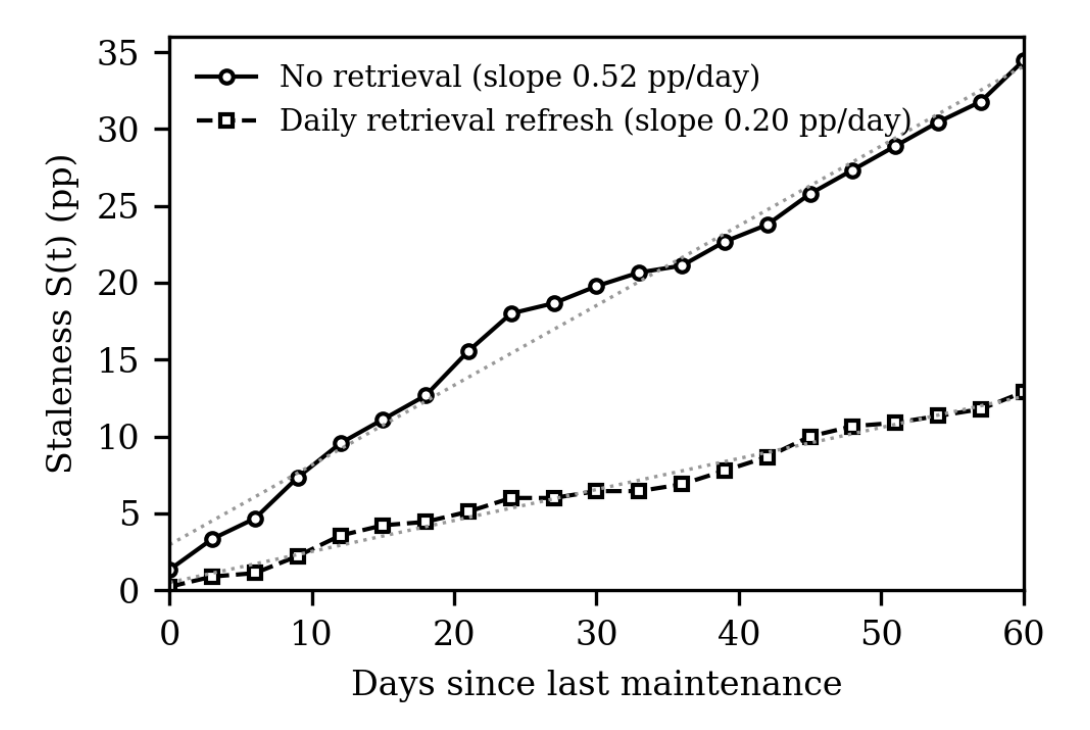
\includegraphics[width=10.5 cm]{fig1}
\caption{Error on the dynamic suite of the deployed Pythia-70M model over 60 days without parametric maintenance, measured every three days (single seed). Dotted lines are least-squares fits. The value at $t=0$ is the residual error of the deployed model, which was trained to at least 95\%, not 100\%, accuracy; staleness $S(t)$ as defined in \eqref{eq:staleness} is the curve minus this intercept, and the fitted slopes are unaffected. Retrieval over a corpus covering 60\% of the drifting facts reduces the fitted slope from 0.52 to 0.20 percentage points per day, an absorbed share of 61\%.\label{fig:staleness}}
\end{figure}

Figure~\ref{fig:staleness} shows the growth of staleness over 60 days of unaddressed drift, measured every three days, with and without retrieval. Both trajectories are well described by the affine form of \eqref{eq:meanstaleness}: OLS gives a slope of 0.519 percentage points per day without retrieval ($R^2=0.987$) and 0.202 percentage points per day with a daily retrieval refresh ($R^2=0.985$), which is precisely the estimation procedure of Section~\ref{sec:estimation}. Over this horizon, 180 drift events are expected, and the expected fraction of distinct dynamic facts that have changed at least once is $1-e^{-180/450}\approx 0.33$ rather than $180/450=0.40$; the affine fit is therefore a local approximation to a process that saturates on longer horizons (Section~\ref{sec:freshness}). The ratio of the two slopes yields a retrieval-absorbed drift share of $\phibar/\gamma=1-0.202/0.519=0.611$, which matches the fraction of dynamic facts indexed in the retrieval store (0.60) to within the resolution of the experiment: retrieval absorbs the share of drift that it covers, and no more, in agreement with the boundedness of the compensator in Section~\ref{sec:ragcontrol}. Substituting this share into \eqref{eq:ragopt} predicts that maintaining the retrieval store lengthens the economically optimal interval between parametric updates by a factor of $1/\sqrt{1-0.611}\approx 1.60$ at any fixed retraining cost, and lowers the optimal staleness threshold by the reciprocal factor, 0.62.

Table~\ref{tab:mechanisms} reports the measured cost, error reduction, and forgetting of three parametric maintenance mechanisms, each applied to the same deployed model after 10 and 30 days of accumulated drift: a localized knowledge edit that fine-tunes only the multilayer perceptron (MLP) block of a single transformer layer on the facts of those entities for which a drift event was logged, a low-rank adaptation (LoRA, rank 16) trained on all dynamic facts without any replay of the static suite, and a full fine-tune of all parameters on all current facts. Costs are computed under the trainable-parameter accounting \eqref{eq:costtp}, as six times the number of trainable parameters times the number of tokens processed, and normalized so that a full fine-tune equals 1000 cost units.

\begin{table}[H]
\caption{Measured cost, error reduction, and forgetting of three maintenance mechanisms on Pythia-70M.\label{tab:mechanisms}}
\small
\begin{tabularx}{\textwidth}{LLCCC}
\toprule
\textbf{Mechanism} & \textbf{Trainable Subset} & \textbf{Cost, \eqref{eq:costtp} (Units)} & \textbf{Error Before} \boldmath{$\to$} \textbf{After (pp)} & \textbf{Change in Retention Error (pp)}\\
\midrule
Localized edit & MLP block of one layer (entities with logged drift) & 14.0 & 17.4 $\to$ 13.8 & $-2.0$\\
LoRA ($r=16$, no replay) & Low-rank adapters, all layers & 2.6 & 17.4 $\to$ 24.4 & $+11.0$\\
Full fine-tune & All parameters & 1000 & 17.4 $\to$ 5.7 & $-2.0$\\
\bottomrule
\end{tabularx}
\noindent{\footnotesize{Values are averaged over interventions applied after 10 and 30 days of accumulated drift. Costs are normalized so that a full fine-tune equals 1000 units (about $5.1\times 10^{13}$ FLOP). Error is the sum of staleness on the dynamic suite and error on the static retention suite, i.e., the degradation index $X$ of \eqref{eq:degradation} plus the residual error of the deployed model. A change of $-2.0$ pp corresponds to three of the 150 retention facts and is within single-seed noise.}}
\end{table}

Two of the three mechanisms behave as the framework anticipates. The full fine-tune is the most effective, reducing total error from 17.4 to 5.7 percentage points, and by far the most expensive at 1000 cost units. The localized edit reduces total error from 17.4 to 13.8 percentage points at 14 cost units under the trainable-parameter accounting. Neither mechanism caused forgetting: retention-suite error fell by 2.0 percentage points under both, a change of three facts that we attribute to single-seed noise rather than to a genuine improvement. Per unit of trainable-parameter compute, the edit therefore removes considerably more error than the full fine-tune. This is the concrete expression of the argument in Section~\ref{sec:constrained} that a displacement confined to a small, sparse subspace purchases plasticity at negligible stability cost. This comparison, however, overstates the edit's compute advantage: the forward-inclusive accounting \eqref{eq:cost} also charges the edit a forward pass through all parameters and a backward pass down to the edited layer for every processed token, so its advantage under that accounting is smaller. Together these two mechanisms satisfy the ordering assumed in condition (ii) of Proposition~\ref{prop:monotone}: the more aggressive action is both more effective and more expensive.

The low-rank adaptation does not. Although it is the cheapest of the three mechanisms at 2.6 cost units under the trainable-parameter accounting, it raises total error from 17.4 to 24.4 percentage points and induces 11.0 percentage points of forgetting on the static retention suite, with a large spread between the 10-day and 30-day interventions. In the language of Section~\ref{sec:pareto}, an unreplayed adapter trained at a comparatively high learning rate on the drifting facts alone produces a displacement whose direction is not orthogonal to the high-curvature directions of the pre-update loss on the static facts, so the update lands on the steep part of the stability--plasticity frontier; the fact that the adapter is low-rank bounds $\|\D\|_0$ but does not by itself constrain the Fisher-weighted norm $\D^{\top}F\D$ in \eqref{eq:constrained}. This is an empirical instance of the caveat raised in Section~\ref{sec:structdiscussion}: parameter efficiency is not the same as low forgetting. The measured costs also break the nominal order of \eqref{eq:actions} in a second way, since the PEFT action is cheaper than the knowledge edit rather than more expensive. The LoRA action is nevertheless harmless to the policy, because it is dominated by the no-op: it costs more, forgets more, and leaves the model with a higher total error than doing nothing. Since the relative value function is non-decreasing in the degradation index (Proposition~\ref{prop:monotone}, whose monotonicity part requires only condition (i)), an action whose one-step cost is higher and whose next state is stochastically larger than those of the no-op is never strictly preferred to it, so an MDP instantiated with the measured parameters never needs to select LoRA. Removing it leaves the ordered set no-op $\prec$ localized edit $\prec$ full fine-tune, which satisfies condition (ii). We report this configuration as measured rather than tuning it away, because it illustrates that the ordering in Proposition~\ref{prop:monotone} is a property to be verified for each candidate mechanism from measurements of the kind in Table~\ref{tab:mechanisms}, not an assumption that can be made on the basis of the mechanism's name.

The case study validates the framework at the level of its measured inputs---affine staleness growth, a retrieval-absorbed share equal to retrieval coverage, and a cost/effectiveness/forgetting profile per mechanism that can be read directly into the action set of Section~\ref{sec:mdp}---on a small model with synthetic drift. Validation at the level of the scheduling decision itself, comparing periodic retraining with the threshold policy of Proposition~\ref{prop:monotone} in closed loop over a long horizon, and replication over multiple seeds and larger models, remain to be done and are discussed in Section~\ref{sec:validation}.

\subsection{Summary of Findings}

The analytical and numerical results of Sections~\ref{sec:staleness}--\ref{sec:numerical} can be summarized as six findings. First, under Poisson drift arrivals the optimal interval between retraining events grows with the square root of the retraining cost and shrinks with the square root of the drift intensity, while the tolerated staleness level grows with both (Section~\ref{sec:renewal}). Second, whether a memoryless threshold policy is adequate is hypothesized to depend on the aging property of the drift-arrival distribution, with opposite prescriptions for a long quiet interval under DMRL and under IMRL (Sections~\ref{sec:hazard} and~\ref{sec:hazardsens}). Third, forgetting can be expressed as a Fisher-weighted quadratic form in the parameter displacement, so the stability--plasticity trade-off becomes a Pareto frontier whose steepness depends on the alignment between the update direction and the high-curvature directions of the pre-update loss; lower forgetting per event lowers the optimal cost rate and shortens the optimal interval (Section~\ref{sec:forgetting}). Fourth, under stochastic-monotonicity and submodularity conditions on the transition kernel, an optimal policy over a graduated menu of maintenance actions escalates through a sequence of degradation thresholds (Proposition~\ref{prop:monotone}). Fifth, retrieval augmentation lengthens the optimal interval between parametric updates by the factor $1/\sqrt{1-\phibar/\gamma}$, dominates parametric maintenance alone exactly when its upkeep cost satisfies \eqref{eq:blendcond}, and cannot substitute for parametric maintenance when the drift is not retrievable (Section~\ref{sec:rag}). Sixth, on a public 70M-parameter model with synthetic drift, measured staleness grows affinely with a retrieval-absorbed share equal to retrieval coverage, a localized edit removes more error per unit of trainable-parameter compute than full fine-tuning, and an unreplayed low-rank adaptation violates the action ordering of Proposition~\ref{prop:monotone} and is dominated by the no-op (Section~\ref{sec:casestudy}). The first five findings are derived from the model and illustrated with stylized parameters; the sixth is a controlled measurement on a small model rather than a validation against deployment data.

%-----------------------------------------------------------------
\section{Managerial Implications}\label{sec:managerial}

The framework is stated in the language of stochastic control, but its results answer questions that managers responsible for deployed LLMs face directly: how much to budget for maintenance, how often to update, which update mechanisms to adopt, how much behavioral regression to tolerate, and whether to invest in retrieval. This section translates the results of Sections~\ref{sec:staleness}--\ref{sec:numerical} into guidelines for those decisions. Table~\ref{tab:managerial} summarizes the mapping.

\begin{table}[H]
\caption{Managerial decisions and the results that inform them.\label{tab:managerial}}
\small
\begin{tabularx}{\textwidth}{p{3.1cm}p{3.1cm}L}
\toprule
\textbf{Managerial Decision} & \textbf{Result in This Paper} & \textbf{Practical Guideline}\\
\midrule
How often to update the model & Square-root law \eqref{eq:sqrt} & Set the cadence from measured drift and update cost; a tenfold rise in update cost justifies only about a threefold longer interval\\
\midrule
Which update mechanisms to adopt & Proposition~\ref{prop:monotone}; Table~\ref{tab:mechanisms} & Admit a mechanism to the maintenance menu only after measuring its cost, effectiveness, and forgetting\\
\midrule
How much regression to tolerate & Forgetting constraint \eqref{eq:constrained}; optimum \eqref{eq:forgetopt} & Set the forgetting tolerance and its cost explicitly as governance parameters\\
\midrule
Whether to invest in retrieval & Blending condition \eqref{eq:blendcond} & Invest when retrieval upkeep is below the saving it creates, and only for drift that retrieval can absorb\\
\midrule
What to monitor & Estimation procedure of Section~\ref{sec:estimation} & Track staleness and retention error on fixed evaluation suites across every maintenance cycle\\
\bottomrule
\end{tabularx}
\end{table}

\subsection{Treat Model Maintenance as a Budgeted Operations Decision}

The first implication is organizational rather than technical. In many organizations, the decision to update a deployed model is made by the team that built it, on a calendar inherited from software release cycles or in response to a visible incident. The objective \eqref{eq:objective} shows that the decision in fact trades off three costs that are usually owned by different parts of the organization: the operational loss from an outdated model, which falls on the business units that use it; the compute and engineering cost of an update, which falls on the platform or MLOps team; and the cost of behavioral regressions, which falls on risk, compliance, and customer-facing functions. The coefficients $\alpha$ and $\beta$ and the tolerance $\Gmax$ are therefore not technical hyperparameters but statements of organizational priorities. Making them explicit, and assigning ownership of each, turns model maintenance from an engineering routine into a budgeted operations decision that can be reviewed and defended in the same way as other IT maintenance expenditures.

\subsection{Size the Maintenance Cadence with the Square-Root Rule}

The square-root law of Section~\ref{sec:renewal} gives managers a simple rule for budgeting. Because the optimal interval grows only with the square root of the update cost, moving to a model that is ten times more expensive to update justifies an update interval only about three times longer, not ten times longer. Conversely, if monitoring shows that the environment around the model is changing four times faster than before, the interval should be halved, not quartered. Two common heuristics are therefore miscalibrated: stretching the update cycle in proportion to update cost, which leaves expensive models stale for too long, and matching the update frequency to the drift rate, which overreacts to changes in the environment. The same law also bounds the value of negotiating lower update costs, for example with a cloud provider or model vendor: halving the cost of an update lowers the optimal cost rate by only about 29\%, because the organization responds by updating more often.

\subsection{Build a Graduated Maintenance Menu and Verify Each Mechanism}

Proposition~\ref{prop:monotone} supports a policy of escalation: when degradation is small, apply the lightest mechanism that restores the model, and reserve full retraining for high degradation. For managers, this means that maintenance capability should be built as a menu---targeted knowledge editing, parameter-efficient fine-tuning, and full retraining---with escalation thresholds agreed in advance, rather than as a single retraining pipeline. The case study adds an important qualification. A mechanism's name does not guarantee its place in the menu: the unreplayed low-rank adapter was the cheapest mechanism tested but made the model worse than doing nothing. Before a mechanism is adopted, it should pass an acceptance test that measures its cost, its error reduction, and its forgetting on a fixed retention suite, in the form of Table~\ref{tab:mechanisms}. This acceptance test is the maintenance counterpart of the regression testing that software organizations already apply to code changes, and it can be embedded in the same change-management process.

\subsection{Govern Forgetting Explicitly}

Every parameter update risks degrading behavior that users and regulators already rely on, and the alignment tax documented by Ouyang et al.~\cite{Ouyang2022} shows that this risk extends to safety and policy behavior. The constrained update problem \eqref{eq:constrained} makes the organization's tolerance for such regressions an explicit quantity, $\Gmax$, that can be set by risk owners, recorded, and audited, instead of being left implicit in a training hyperparameter. The optimum \eqref{eq:forgetopt} adds two points that are useful in governance discussions. First, residual forgetting imposes a permanent cost, $\alpha G$, that no choice of update frequency can remove, so a cheap mechanism that forgets can be more expensive in the long run than a costly one that does not. Second, mechanisms that forget less make each update less costly and therefore justify updating more often, so investment in safer update mechanisms pays off partly through a fresher model rather than through fewer updates.

\subsection{Invest in Retrieval Where Drift Is Factual}

Retrieval augmentation is often presented as an alternative to retraining. The analysis of Section~\ref{sec:rag} and the case study support a more precise position. Retrieval absorbs the share of drift that its corpus covers and no more: in the case study, a store covering 60\% of the drifting facts absorbed 61\% of the staleness growth. It therefore substitutes for parametric maintenance only for drift that consists of facts that can be looked up, not for changes in required reasoning, output formats, or policy norms. Condition \eqref{eq:blendcond} gives managers an investment test: maintaining a retrieval store is worthwhile when its upkeep cost per unit time is lower than the reduction in the optimal parametric maintenance cost that it produces. Because that reduction grows with the absorbed share, the coverage of the retrieval corpus over the facts that actually change is the key operational metric for a retrieval investment, and it should be monitored as part of the maintenance program rather than assumed once the system is deployed.

\subsection{Invest in Monitoring Before Optimizing}

All of the guidelines above depend on estimates of the drift rate, the update costs, and the forgetting of each mechanism, and these can only be obtained from a monitoring program. The estimation procedure of Section~\ref{sec:estimation} requires fixed evaluation suites for the drifting knowledge and for retained behavior, applied consistently before and after every maintenance event, and records of when drift was detected. Organizations that change their evaluation methods between maintenance cycles lose the ability to estimate these quantities. Until enough cycles have been observed, managers should rely on the qualitative results---the square-root sensitivity of the interval, the escalation structure, and the partial nature of retrieval substitution---which hold regardless of the exact parameter values, and move to numerically optimized policies as monitoring data accumulate.

%-----------------------------------------------------------------
\section{Limitations and Future Work}\label{sec:limitations}

\subsection{Identifiability and Data Requirements}

A practical limitation, distinct from the modeling assumptions of Section~\ref{sec:assumptions}, concerns identifiability: the estimation procedure of Section~\ref{sec:estimation} requires repeated observation of full maintenance cycles---staleness accumulating from a reset point, a maintenance event, and a subsequent reset---in order to fit even the simplest affine decay model, and organizations that maintain their models very infrequently, or that have changed maintenance mechanism or monitoring methodology between cycles, may simply lack the historical data needed to estimate $\gamma$, let alone the richer hazard-rate structure of Section~\ref{sec:hazard}, with any precision. In such data-poor settings, the qualitative comparative statics derived analytically in Sections~\ref{sec:staleness}--\ref{sec:mdp}---for instance, the square-root sensitivity of the optimal interval to cost and to drift intensity---are arguably of more immediate practical value than any point estimate of the optimal threshold itself, since the former are robust, structural predictions while the latter is only as reliable as the (possibly very limited) historical record used to calibrate it.

\subsection{Scalar Accuracy and Multi-Task Heterogeneity}

Assumption A1 treats task-relevant accuracy $A(\theta,w)$ as a single scalar and adds staleness and forgetting in the degradation index, but a deployed LLM is evaluated by its users along many largely independent axes---factual accuracy, coding ability, safety compliance, stylistic preference---each of which may drift at a different rate and respond differently to a given maintenance mechanism. A vector-valued extension of Sections~\ref{sec:formal}--\ref{sec:mdp}, in which staleness and forgetting are tracked per task cluster and the maintenance action space is allowed to target clusters selectively (as targeted knowledge editing already does implicitly~\cite{WangS2024,Zhang2024}), is a natural next step and would allow the threshold-policy result of Section~\ref{sec:mdp} to be tested for robustness under a genuinely multi-objective cost structure, in the manner of multi-component maintenance models in reliability theory~\cite{Dekker1997}.

\subsection{Endogeneity of the World Process}

Assumption A2 holds that the world process $w_t$ evolves independently of the deployed model's own outputs. This assumption is already strained by the growing presence of LLM-generated text in the corpora used to evaluate and retrain subsequent models, which introduces a feedback loop between a model's maintenance history and the very drift process it is trying to track; formalizing this feedback---for instance, by allowing the drift-event rate $\lambda$ in Section~\ref{sec:staleness} to depend on cumulative prior deployment---is left for future work and would connect this paper's renewal-theoretic framework to the broader literature on degradation induced by training on model-generated data~\cite{Shumailov2024}.

\subsection{Parameter Estimation Under Non-Stationarity}

The estimation procedure sketched in Section~\ref{sec:estimation} assumes that the parameters $\eta$, $\lambda$, $\mu_M$ governing drift are themselves stable across the observation window used to estimate them; if these parameters are themselves slowly time-varying (a plausible scenario, since the rate at which the world changes is not itself constant), a more sophisticated online, possibly Bayesian, estimation scheme would be required, and the fixed-threshold and even the regime-dependent policies of Sections~\ref{sec:staleness}--\ref{sec:mdp} would need to be re-derived as adaptive-control rather than fixed-parameter optimal-control problems.

\subsection{Empirical Validation}\label{sec:validation}

This paper is primarily a mathematical modeling contribution: its numerical illustrations in Sections~\ref{sec:qualitative} and~\ref{sec:hazardsens} are chosen for interpretability, and the case study of Section~\ref{sec:casestudy}, while it uses a real pretrained model, is a controlled experiment on a 70M-parameter checkpoint with synthetic drift, a single random seed, and a closed set of eight candidate answers per fact, none of which reflect the scale or the open-ended evaluation of a production deployment. The cost comparison in that study also depends on the FLOP accounting used (Section~\ref{sec:cost}). A natural and important next step is to instantiate the model---the staleness-decay parameters of Section~\ref{sec:staleness}, the Fisher-information-based forgetting model of Section~\ref{sec:forgetting}, and the action-cost structure of Section~\ref{sec:mdp}---against telemetry from an actual production LLM deployment, and to test the central falsifiable predictions of the framework: the square-root relationship between retraining cost and optimal interval (Section~\ref{sec:renewal}), the diminishing sensitivity of the optimum to drift intensity (Section~\ref{sec:qualitative}), the opposite effects of forgetting and of drift intensity on the optimal interval (Sections~\ref{sec:forgetrenewal} and~\ref{sec:renewal}), the threshold-escalation structure of the optimal multi-action policy (Proposition~\ref{prop:monotone}), and the partial-substitution relationship between retrieval augmentation and parametric maintenance frequency (Section~\ref{sec:blending}).

%-----------------------------------------------------------------
\section{Conclusions}\label{sec:conclusions}

This paper has argued that the maintenance of a deployed large language model---the recurring decision of when, how much, and by which mechanism to update it---is a condition-based maintenance problem for a deteriorating system, and can be given a coherent mathematical treatment that unifies previously separate strands of the continual-learning, concept-drift, and MLOps literatures under a single renewal-reward optimization objective drawn from reliability theory. Modeling knowledge staleness as a shock-and-wear process driven by random drift events, modeling update-induced forgetting as a Fisher-information-weighted constraint on parameter displacement in the tradition of EWC~\cite{Kirkpatrick2017} and of imperfect maintenance~\cite{Pham1996}, and modeling the joint scheduling and mechanism-selection decision as an MDP yields both closed-form results in restricted cases---most notably a square-root relationship between retraining cost, drift intensity, and the economically optimal maintenance interval, and the result that lower forgetting per event warrants more frequent maintenance---and a structural theorem establishing that, under stochastic-monotonicity and submodularity conditions, an optimal policy over a graduated menu of maintenance mechanisms takes the form of an escalating sequence of degradation thresholds. The framework further shows that retrieval-augmented generation is properly understood not as an alternative to parametric maintenance but as a feedback compensator that partially and boundedly substitutes for it, and gives a closed-form condition under which the blend is worth its upkeep. A case study on a public pretrained model confirms the affine staleness growth and the retrieval-coverage bound that the framework assumes, and, by exhibiting a parameter-efficient update that violates the monotone action ordering, demonstrates that the framework's conditions are measurable properties of candidate mechanisms rather than articles of faith. Beyond its specific formulas, the central claim of this paper is methodological: that treating LLM maintenance as a first-class, jointly optimized stochastic control problem---rather than as a collection of separately tuned heuristics for drift detection, forgetting mitigation, and cost control---both explains qualitative patterns already visible in the empirical literature and yields new, falsifiable predictions that can guide the design of maintenance policies for future deployed systems.

%=================================================================
% Back matter (MDPI required statements). Please verify each one.
\vspace{6pt}

\funding{This research received no external funding.} % TODO: confirm, or replace with funder name and grant number

\institutionalreview{Not applicable.}

\informedconsent{Not applicable.}

\dataavailability{The data and code supporting the case study in Section~\ref{sec:casestudy} are available from the author upon reasonable request.} % TODO: replace with a public repository link if available

% MDPI requires disclosure of generative-AI use beyond grammar/formatting edits. Uncomment and complete if applicable.
%\acknowledgments{During the preparation of this manuscript, the author used [tool name, version] for the purposes of [description of use]. The author has reviewed and edited the output and takes full responsibility for the content of this publication.}

\conflictsofinterest{The author declares no conflicts of interest.}

\abbreviations{Abbreviations}{
The following abbreviations are used in this manuscript:
\\

\noindent
\begin{tabular}{@{}ll}
CBM & Condition-based maintenance\\
DMRL & Decreasing mean residual life\\
EWC & Elastic weight consolidation\\
FLOP & Floating-point operations\\
IMRL & Increasing mean residual life\\
KME & Knowledge-based model editing\\
LLM & Large language model\\
LoRA & Low-rank adaptation\\
MDP & Markov decision process\\
MLOps & Machine-learning operations\\
MLP & Multilayer perceptron\\
OLS & Ordinary least squares\\
PEFT & Parameter-efficient fine-tuning\\
RAG & Retrieval-augmented generation\\
RLHF & Reinforcement learning from human feedback
\end{tabular}
}

%=================================================================
\begin{adjustwidth}{-\extralength}{0cm}

\reftitle{References}

% References are numbered in order of first citation in the text (MDPI style).
\begin{thebibliography}{999}

\bibitem[Pham and Wang(1996)]{Pham1996}
Pham, H.; Wang, H. Imperfect maintenance. {\em Eur. J. Oper. Res.} {\bf 1996}, {\em 94}, 425--438. \url{https://doi.org/10.1016/S0377-2217(96)00099-9}

\bibitem[Jardine et~al.(2006)]{Jardine2006}
Jardine, A.K.S.; Lin, D.; Banjevic, D. A review on machinery diagnostics and prognostics implementing condition-based maintenance. {\em Mech. Syst. Signal Process.} {\bf 2006}, {\em 20}, 1483--1510. \url{https://doi.org/10.1016/j.ymssp.2005.09.012}

\bibitem[van Noortwijk(2009)]{vanNoortwijk2009}
van Noortwijk, J.M. A survey of the application of gamma processes in maintenance. {\em Reliab. Eng. Syst. Saf.} {\bf 2009}, {\em 94}, 2--21. \url{https://doi.org/10.1016/j.ress.2007.03.019}

\bibitem[Wang(2002)]{Wang2002}
Wang, H. A survey of maintenance policies of deteriorating systems. {\em Eur. J. Oper. Res.} {\bf 2002}, {\em 139}, 469--489. \url{https://doi.org/10.1016/S0377-2217(01)00197-7}

\bibitem[Lu et~al.(2019)]{Lu2019}
Lu, J.; Liu, A.; Dong, F.; Gu, F.; Gama, J.; Zhang, G. Learning under concept drift: A review. {\em IEEE Trans. Knowl. Data Eng.} {\bf 2019}, {\em 31}, 2346--2363. \url{https://doi.org/10.1109/TKDE.2018.2876857}

\bibitem[Mahadevan and Mathioudakis(2023)]{Mahadevan2023}
Mahadevan, A.; Mathioudakis, M. Cost-effective retraining of machine learning models. {\em arXiv} {\bf 2023}, arXiv:2310.04216. \url{https://doi.org/10.48550/arXiv.2310.04216}

\bibitem[Hoffmann et~al.(2022)]{Hoffmann2022}
Hoffmann, J.; Borgeaud, S.; Mensch, A.; Buchatskaya, E.; Cai, T.; Rutherford, E.; de~Las~Casas, D.; Hendricks, L.A.; Welbl, J.; Clark, A.; et~al. Training compute-optimal large language models. {\em arXiv} {\bf 2022}, arXiv:2203.15556. \url{https://doi.org/10.48550/arXiv.2203.15556}

\bibitem[Kaplan et~al.(2020)]{Kaplan2020}
Kaplan, J.; McCandlish, S.; Henighan, T.; Brown, T.B.; Chess, B.; Child, R.; Gray, S.; Radford, A.; Wu, J.; Amodei, D. Scaling laws for neural language models. {\em arXiv} {\bf 2020}, arXiv:2001.08361. \url{https://doi.org/10.48550/arXiv.2001.08361}

\bibitem[Kirkpatrick et~al.(2017)]{Kirkpatrick2017}
Kirkpatrick, J.; Pascanu, R.; Rabinowitz, N.; Veness, J.; Desjardins, G.; Rusu, A.A.; Milan, K.; Quan, J.; Ramalho, T.; Grabska-Barwinska, A.; et~al. Overcoming catastrophic forgetting in neural networks. {\em Proc. Natl. Acad. Sci. USA} {\bf 2017}, {\em 114}, 3521--3526. \url{https://doi.org/10.1073/pnas.1611835114}

\bibitem[Luo et~al.(2023)]{Luo2023}
Luo, Y.; Yang, Z.; Meng, F.; Li, Y.; Zhou, J.; Zhang, Y. An empirical study of catastrophic forgetting in large language models during continual fine-tuning. {\em arXiv} {\bf 2023}, arXiv:2308.08747. \url{https://doi.org/10.48550/arXiv.2308.08747}

\bibitem[Shi et~al.(2024)]{Shi2024}
Shi, H.; Xu, Z.; Wang, H.; Qin, W.; Wang, W.; Wang, Y.; Wang, Z.; Ebrahimi, S.; Wang, H. Continual learning of large language models: A comprehensive survey. {\em arXiv} {\bf 2024}, arXiv:2404.16789. \url{https://doi.org/10.48550/arXiv.2404.16789}

\bibitem[Wang et~al.(2024)]{WangS2024}
Wang, S.; Zhu, Y.; Liu, H.; Zheng, Z.; Chen, C.; Li, J. Knowledge editing for large language models: A survey. {\em ACM Comput. Surv.} {\bf 2024}, {\em 57}, 1--37. \url{https://doi.org/10.1145/3698590}

\bibitem[Zhang et~al.(2024)]{Zhang2024}
Zhang, N.; Yao, Y.; Tian, B.; Wang, P.; Deng, S.; Wang, M.; Xi, Z.; Mao, S.; Zhang, J.; Ni, Y.; et~al. A comprehensive study of knowledge editing for large language models. {\em arXiv} {\bf 2024}, arXiv:2401.01286. \url{https://doi.org/10.48550/arXiv.2401.01286}

\bibitem[Gao et~al.(2023)]{Gao2023}
Gao, Y.; Xiong, Y.; Gao, X.; Jia, K.; Pan, J.; Bi, Y.; Dai, Y.; Sun, J.; Wang, M.; Wang, H. Retrieval-augmented generation for large language models: A survey. {\em arXiv} {\bf 2023}, arXiv:2312.10997. \url{https://doi.org/10.48550/arXiv.2312.10997}

\bibitem[Wu et~al.(2024)]{Wu2024}
Wu, T.; Luo, L.; Li, Y.-F.; Pan, S.; Vu, T.-T.; Haffari, G. Continual learning for large language models: A survey. {\em arXiv} {\bf 2024}, arXiv:2402.01364. \url{https://doi.org/10.48550/arXiv.2402.01364}

\bibitem[Williams et~al.(2026)]{Williams2026}
Williams, E.; Sinha, T.; Lyttle, M.; Kanagasingam, Y. Optimising retraining frequency for a paediatric emergency department admission prediction model: Development and temporal validation using real-world data. {\em Emerg. Med. Australas.} {\bf 2026}, {\em 38}, e70271. \url{https://doi.org/10.1111/1742-6723.70271}

\bibitem[Barlow and Proschan(1996)]{Barlow1965}
Barlow, R.E.; Proschan, F. {\em Mathematical Theory of Reliability}; Society for Industrial and Applied Mathematics: Philadelphia, PA, USA, 1996. \url{https://doi.org/10.1137/1.9781611971194}

\bibitem[Beytur et~al.(2025)]{Beytur2025}
Beytur, H.B.; de~Veciana, G.; Vikalo, H.; Chan, K.S. Optimal resource allocation for ML model training and deployment under concept drift. {\em arXiv} {\bf 2025}, arXiv:2512.12816. \url{https://doi.org/10.48550/arXiv.2512.12816}

\bibitem[Ross(1996)]{Ross1996}
Ross, S.M. {\em Stochastic Processes}, 2nd ed.; John Wiley \& Sons: New York, NY, USA, 1996.

\bibitem[Bertsekas(2017)]{Bertsekas2017}
Bertsekas, D.P. {\em Dynamic Programming and Optimal Control}, 4th ed.; Athena Scientific: Belmont, MA, USA, 2017; Volume~I.

\bibitem[Puterman(1994)]{Puterman1994}
Puterman, M.L. {\em Markov Decision Processes: Discrete Stochastic Dynamic Programming}; John Wiley \& Sons: New York, NY, USA, 1994. \url{https://doi.org/10.1002/9780470316887}

\bibitem[Vaswani et~al.(2017)]{Vaswani2017}
Vaswani, A.; Shazeer, N.; Parmar, N.; Uszkoreit, J.; Jones, L.; Gomez, A.N.; Kaiser, {\L}.; Polosukhin, I. Attention is all you need. {\em Adv. Neural Inf. Process. Syst.} {\bf 2017}, {\em 30}, 5998--6008. \url{https://doi.org/10.48550/arXiv.1706.03762}

\bibitem[Brown et~al.(2020)]{Brown2020}
Brown, T.; Mann, B.; Ryder, N.; Subbiah, M.; Kaplan, J.D.; Dhariwal, P.; Neelakantan, A.; Shyam, P.; Sastry, G.; Askell, A.; et~al. Language models are few-shot learners. {\em Adv. Neural Inf. Process. Syst.} {\bf 2020}, {\em 33}, 1877--1901. \url{https://doi.org/10.48550/arXiv.2005.14165}

\bibitem[Husz\'ar(2018)]{Huszar2018}
Husz\'ar, F. Note on the quadratic penalties in elastic weight consolidation. {\em Proc. Natl. Acad. Sci. USA} {\bf 2018}, {\em 115}, E2496--E2497. \url{https://doi.org/10.1073/pnas.1717042115}

\bibitem[Kunstner et~al.(2019)]{Kunstner2019}
Kunstner, F.; Balles, L.; Hennig, P. Limitations of the empirical Fisher approximation for natural gradient descent. {\em Adv. Neural Inf. Process. Syst.} {\bf 2019}, {\em 32}. \url{https://doi.org/10.48550/arXiv.1905.12558}

\bibitem[Ouyang et~al.(2022)]{Ouyang2022}
Ouyang, L.; Wu, J.; Jiang, X.; Almeida, D.; Wainwright, C.; Mishkin, P.; Zhang, C.; Agarwal, S.; Slama, K.; Ray, A.; et~al. Training language models to follow instructions with human feedback. {\em Adv. Neural Inf. Process. Syst.} {\bf 2022}, {\em 35}, 27730--27744. \url{https://doi.org/10.52202/068431-2011}

\bibitem[Poenaru-Olaru et~al.(2025)]{PoenaruOlaru2025}
Poenaru-Olaru, L.; Sallou, J.; Cruz, L.; Rellermeyer, J.S.; van Deursen, A. Sustainable machine learning retraining: Optimizing energy efficiency without compromising accuracy. {\em arXiv} {\bf 2025}, arXiv:2506.13838. \url{https://doi.org/10.48550/arXiv.2506.13838}

\bibitem[Topkis(1998)]{Topkis1998}
Topkis, D.M. {\em Supermodularity and Complementarity}; Princeton University Press: Princeton, NJ, USA, 1998. \url{https://doi.org/10.1515/9781400822539}

\bibitem[Ji et~al.(2023)]{Ji2023}
Ji, Z.; Lee, N.; Frieske, R.; Yu, T.; Su, D.; Xu, Y.; Ishii, E.; Bang, Y.J.; Madotto, A.; Fung, P. Survey of hallucination in natural language generation. {\em ACM Comput. Surv.} {\bf 2023}, {\em 55}, 1--38. \url{https://doi.org/10.1145/3571730}

\bibitem[Dekker et~al.(1997)]{Dekker1997}
Dekker, R.; Wildeman, R.E.; van~der Duyn~Schouten, F.A. A review of multi-component maintenance models with economic dependence. {\em Math. Methods Oper. Res.} {\bf 1997}, {\em 45}, 411--435. \url{https://doi.org/10.1007/BF01194788}

\bibitem[Shumailov et~al.(2024)]{Shumailov2024}
Shumailov, I.; Shumaylov, Z.; Zhao, Y.; Papernot, N.; Anderson, R.; Gal, Y. AI models collapse when trained on recursively generated data. {\em Nature} {\bf 2024}, {\em 631}, 755--759. \url{https://doi.org/10.1038/s41586-024-07566-y}

\end{thebibliography}

\PublishersNote{}
\end{adjustwidth}
\end{document}
